\documentclass[thesis.tex]{subfiles}
\begin{document}
In the previous chapter the classical (or standard) residual error estimator is introduced as the driver for the
adaptive finite element method (AFEM). This results in an optimal algorithm, i.e. the adaptive meshes
generated by this method provide the highest possible convergence rate. Unfortunately, this asymptotic result
is a bit unfortunate for practical purposes due to the unknown constants. In practice
one would like to know \emph{when} to stop iterating, i.e. when the approximation error is small enough --- say
below some threshold. 

Another problem of the classical residual error estimator is that it is not polynomial-degree-robust; 
the constants depend on $p$, the degree of the finite element solutions. This becomes an issue
when considering \emph{hp}-FEM, a version of AFEM where the polynomial degree can also vary
per simplex. For \emph{hp}-FEM one would like an estimator with a constant independent of the polynomial degree
used in the finite element space.

Conveniently, there are error estimators that suffer less from these constants problems. Recently quite
some research interest has been shown for such constant-free estimators. One of these estimators is the
\emph{equilibrated residual error estimator} also called the \emph{equilibrated flux estimator} or the \emph{Braess-Sch\"oberl estimator}
\cite{braessequil, braessequilrobust,ernequil}.
In this chapter we will introduce this estimator --- which we will refer to as the equilibrated flux estimator --- alongside some results, and prove that AFEM driven 
by this estimator is again optimal. 

For simplicity we restrict ourself to the Poisson problem \eqref{eq:poisson} on a two-dimensional domain $\O \subset \R^2$,
with a right hand side $f \in L^2(\O)$. For some conforming triangulation~$\T$ of the domain we consider $\VV(\T)$: the (Lagrange) finite
element space of degree $p\geq 1$. We assume each triangulation to be uniformly shape regular, i.e. $\sup_{K \in \T} h_K/p_K \leq \kappa$ for
some shape regularity constant $\kappa$.
The Galerkin approximation (discrete solution) is denoted by $U \in \VV(\T)$.
If we do not need to stress dependence on the triangulation, we also write $\VV$ for the finite element space.
\section{Prager and Synge}
The so-called equilibrated flux estimators are based on the fundamental theorem of Prager and Synge \cite{prager}. 
For this we need the space $H(\div; \Omega)$ as defined in \ref{def:hdiv}. Vector-valued functions will be underlined
to emphasise this characteristic.
\begin{thm}[Prager and Synge]
  \label{thm:prager}
  Let $u \in H_0^1(\O)$ be the exact solution of the Poisson problem with a right hand side $f \in L^2(\O)$. 
  For a flux $\v{\sigma} \in H(\div; \O)$ satisfying the equilibrium condition $\div \v{\sigma} + f = 0$ in $L^2$-sense, there holds
\[
  \norm{\nabla u - \nabla v}^2_{\O} + \norm{\nabla u - \v{\sigma}}^2_{\O} = \norm{\nabla v - \v{\sigma}}^2_{\O} \quad \forall v \in H_0^1(\O).
\]
\end{thm}
\begin{proof}
  Applying the divergence theorem \eqref{thm:divergence} yields
  \begin{align*}
    &\int_\O  \left(\nabla u - \v{\sigma}\right) \cdot \nabla \left( u -  v\right)  \, \dif x \\ 
    =  - &\int_\O \left(u - v\right) \,  \div \left (\nabla u - \v{\sigma}\right) \dif x + \int_{\partial \O} (u - v) \left( \nabla u \cdot n - \v{\sigma} \cdot n\right) \dif s  = 0,
  \end{align*}
  since from the assumptions  $\Delta u = -f = \div \v{\sigma}$ in $\O$, and $u - v = 0$ on $\partial \O$.
  From this orthogonality relation and Pythagoras' identity we may conclude that
  \[
    \norm{\nabla(u-v)}^2_{\O} + \norm{\nabla u - \v{\sigma}}^2_{\O} = \norm{ -\nabla (u-v) + \nabla u - \v{\sigma}}^2_{\O},
  \]
  which equals the asserted.
\end{proof}
For a flux $\vsig$ satisfying the equilibrium condition we obtain an 
\emph{reliable} constant-free estimator by replacing $v$ with the discrete solution $U$ in the previous theorem:
\begin{equation}
  \label{eq:synest}
  \enorm{u - U}_{\O}^2 =  \norm{\nabla u - \nabla U }^2_{\O} \leq \norm{\nabla U - \vsig}^2_{\O}.
\end{equation}

The question now arises how to construct $\vsig$. In general one would like an estimator to be proportional to the error.
For this, we need the estimator to also be \emph{efficient}: it should provide a lower bound for $\enorm{u -U}_{\O}$, up to
a constant and possibly an oscillation term. The following construction will provide such efficiency.

From now until \S\ref{sec:oscillation} we suppose that $f$ is a piecewise polynomial of degree at most $p-1$ on $\T$, i.e.
\[
  f\in \P_{p-1}^{-1}(\T) := \set{ f \in L^2(\O): f|_K \in \P_{p-1}(K) \quad \forall K \in \T},
\]
and consider the  $p$-th order Raviart-Thomas space $\RT_p(\T)$ defined by:
\begin{align*} 
  \RT_p(K)    &:= \left[ \P_p(K)\right]^2 + \P_p(K)\v{x}, \\
  \RT_p^{-1}(\T) &= \set{ \v{\sigma} \in \left[L^2(\O)\right]^2 : \v{\sigma}|_K \in \RT_p(K) \quad \forall K \in \T},\\
  \RT_p(\T) &:= H(\div; \O) \cap \RT_p^{-1}(\T).
\end{align*}
Evidently fluxes $\v{\sigma} \in \RT_p(K)$ satisfy $\div \v{\sigma} \in \P_p^{-1}(\T)$; the divergence mapping
is even surjective \cite[Prop~2.3.3]{brezzimixed}, and thus $\RT_p(K)$ contains equilibrated fluxes.
 From~\eqref{eq:synest} we then see that 
the sharpest estimator in the Raviart-Thomas space is found by minimizing $\norm{\nabla U - \sigma}$ over all 
fluxes $\v{\sigma} \in \RT_p(\T)$ that are in equilibrium. However,
this global minimization procedure --- equivalent to the mixed finite element solution \cite{braess2007finite} --- 
is too expensive for computation of an error estimate.

To overcome this problem, Braess and Sch\"oberl \cite{braessequil} propose minimizing local problems instead; a procedure
called \emph{equilibration}.

\section{Equilibration} 
Instead of directly constructing the flux $\v{\sigma}$, the difference $\v{\sigma}^\triangle := \nabla U -  \v{\sigma}$ is considered.
We still assume that $f$ belongs to the broken polynomial space $\P_{p-1}^{-1}(\T)$, as this avoids the effect of
data oscillation.  The flux $\v{\sigma}$ will be constructed in $\RT_p(\T)$; the correction~$\vsig^\triangle$ must 
therefore belong to the broken Raviart-Thomas space $\RT_p^{-1}(\T)$.

Following \cite{ernequil}, we use $\V, \E$ to denote  the set of vertices and edges in the triangulation~$\T$. 
Superscripts  $^{int}$ or $^{bdr}$ are added to indicate restrictions of $\V, \E$ to the interior or the boundary.
For each vertex $a \in \V$, we write $\psi_a$ for the hat function at vertex $a$, 
i.e. the unique function in the linear finite element space
that takes value $1$ at $a$ and vanishes at the other vertices.
These hat functions form a partition of unity: $\sum_{a \in \V} \psi_a \equiv \1$.
The local problems are solved on patches $\omega_a$, given by the star at a vertex $a \in \V$, also being the support of
the hat function $\psi_a$ --- see Figure~\ref{fig:patches} for an illustration. We denote $\gamma_a$ for the union of interior edges touching $a$. 
So for a vertex $a \in \V$ we have
\[
  \omega_a       := \omega\left(\T, a\right) = \bigcup \{ K \in \T : a \in \partial K\},
  \quad \gamma_a := \gamma\left(\T, a\right) = \bigcup \{ e \in \E^{int} : a \in e\}.
\]
Often we are interested in the set of elements $K \in \T$ that make up $\w_a$. We abuse the notation and intuitively write $K \subset \w_a$
under sums as shorthand for $\set{K \in \T : a \in \partial K}$; similarly we write $e \subset \gamma_a$ to mean $\{e \in \E^{int} : a\in e\}$.
 
\begin{figure}
  \centering
  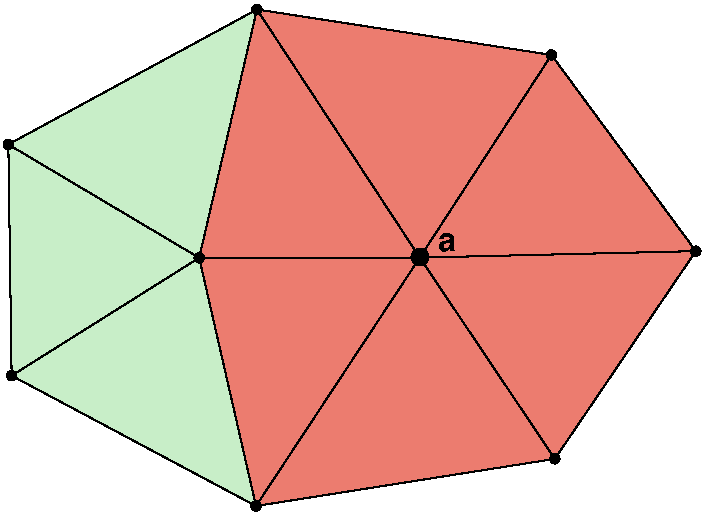
\includegraphics[width=.45\linewidth]{mesh/ex_intpatch.pdf}
  \quad
  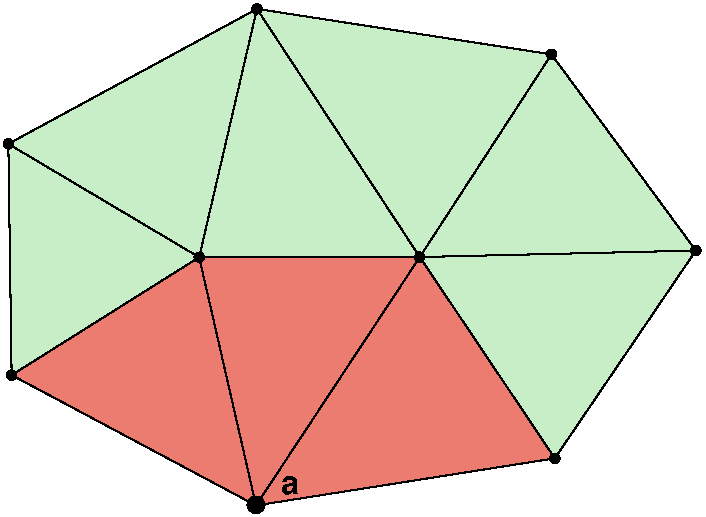
\includegraphics[width=.45\linewidth]{mesh/ex_bdpatch.pdf}
  \caption{Two different type of patches highlighted. The left image displays a patch~$\w_a$  associated to an interior vertex $a$.
  The right image displays a typical patch associated to a boundary vertex.}
  \label{fig:patches}
\end{figure}
  
For each patch $\w_a$ we solve a local problem resulting in a  flux $\vsiga$. 
The total difference flux $\v{\sigma}^\triangle$ is then taken as the sum of local fluxes over these patches, 
\[
  \v{\sigma}^\triangle := \sum_{a \in \V} \vsiga.
\] 
As proposed  in \cite{braessequilrobust}, local fluxes are found by decomposing the residual using the partition of unity. 
Write $r \in H_0^1(\O)'$ for the usual residual defined in \S\ref{sec:afem}, i.e. for $v\in H_0^1(\O)$ 
\[
  \ip{r,v} := a(u - U, v) = \ip{\nabla \left(u - U\right), \nabla v}_\O = \ip{f,v}_\O - \ip{\nabla U,\nabla v}_\O.
\]

For every vertex $a \in \V$ the local residual at $a$ is defined as
\[
  \ip{r_a,v} := \ip{r,\psi_a v} = a(u - U, \psi_a v)_{\w_a}.
\]
The local flux $\vsiga$ is taken from the broken Raviart-Thomas space $\RT_{p}^{-1}(\omega_a)$ such that
\begin{equation}
  \label{eq:defsigma}
  \ip{r_a, v} = - \ip{\v{\sigma_a}, \nabla v}_{\w_a} \quad \forall v \in H^1(\w_a) \cap H_0^1(\O).
\end{equation}
Existence of such a flux $\vsiga$ will be shown at the end of this section.
The residual can be expressed in triangle and edge related terms by applying the divergence theorem.
This leads to the following decomposition:
\begin{equation}
  \label{eq:locdecomp}
  \ip{r_a,v} = \ip{f, \psi_a v}_{\w_a} - \ip{\nabla U, \nabla (\psi_av)}_{\w_a} = \sum_{ K\subset \w_a} \langle{r^T_a, v}\rangle_K + \sum_{ e \subset \gamma_a} \ip{r^e_a, v}_e,
\end{equation}
with $L^2$-inner products over elements $K$ and (lower dimensional) edges $e$, and
\[
  r^T_a := \psi_a \left[ f + \Delta U \right], \quad r^e_a := \psi_a \llbracket \nabla U \rrbracket.
\]
Similarly rewriting $\ip{\v{\sigma_a}, \nabla v}_{\w_a}$ in triangle and edge related terms yields,
\[
  -\ip{\v{\sigma_a}, \nabla v}_{\w_a} = \sum_{K \subset \w_a} \ip{\div \v{\sigma_a}, v}_K + \sum_{ e\subset \gamma_a} \ip{\llbracket \v{\sigma_a}\rrbracket, v} + \ip{\vsiga\cdot n, v}_{\partial \w_a \setminus \partial \O}.
\]
After expanding both sides, we see that \eqref{eq:defsigma} holds if and only if
\begin{equation}
  \label{eq:sigmacons}
  \begin{alignedat}{3}
    \div \v{\sigma_a} &= \psi_a \left [f + \Delta U\right] && \quad\text{in }  K\subset \w_a ,\\
    \llbracket \v{\sigma_a} \rrbracket &= \psi_a \llbracket \nabla U \rrbracket && \quad \text{on } e \subset \gamma_a,\\
    \v{\sigma_a} \cdot n &= 0 &&\quad \text{on } \partial \w_a \setminus \partial \O.
  \end{alignedat}
\end{equation}
To prove that system \eqref{eq:sigmacons} has a solution we make the following observation.
For an interior vertex $a \in \V^{int}$ the hat function $\psi_a$ belongs to the finite element space~$\VV(\T)$. 
Using that $U$ is the Galerkin approximation therefore gives us $\ip{r_a,\1} = \ip{f, \psi_a}_\O - \ip{\nabla U, \nabla \psi_a}_{\O} = 0$.
That is, the local residual vanishes on constant functions.
\begin{thm}
  \label{thm:sigmasolvable}
  There exists a flux $\vsiga \in \RT_{p}^{-1}(\w_a)$ that solves the above system \eqref{eq:sigmacons}.
\end{thm}
\begin{proof}
  We use a (well known) result for Raviart-Thomas elements proved in Lemma~\ref{lem:rtexists}. Namely, 
  for an element $K$ there exists an function $\vtau \in \RT_p(K)$ such that
  \[
    \div \vtau = P_K \, \in \P_p(K), \quad \vtau \cdot n = P_e \in \,\P_p(e) \quad \forall e \subset \partial K,
  \]
  if the polynomials satisfy the compatibility constraint $\int_K P_K = \int_{\partial K} P_e$.
  Notice that the polynomials in \eqref{eq:sigmacons} are of degree $p$, and are thus eligible for in this theorem.

  Fix an interior vertex $a \in \V^{int}$. In this case $\w_a$ is a convex patch, see Figure~\ref{fig:patches}. Let $\set{K_1,\dots,K_n}$ be a numbering
  of the $n$ distinct elements such that $K_i$ and $K_{i+1}$ share an edge, 
  i.e. $K_i \cap K_{i+1} =e_i \in \gamma_a$ for $1 \leq i \leq n-1$. The first and last element also share an edge $K_1 \cap K_n = e_n$,
  because $a$ is an interior vertex. The edges of $K_i$ are thus given by $e_i, e_{i-1}$ and a (patch) boundary edge $\tilde e_i$. 
  For $K_1$ we pick a $\vsign{1}\in \RT_p(K_1)$ that solves 
  \begin{alignat*}{3}
    \div \vsign{1} &= \psi_a \left [f + \Delta U\right] && \quad\text{in }  K_1\subset \w_a ,\\
    \vsign{1} \cdot n  &=-\psi_a \llbracket \nabla U \rrbracket && \quad \text{on } e_n \subset \gamma_a,\\
    \vsign{1} \cdot n  &= 0 && \quad \text{on } \tilde e_1 \subset \partial \w_a,\\
    \vsign{1} \cdot n  &= p_1 && \quad \text{on } e_{1} \subset \gamma_a,
  \end{alignat*}
  with $p_1$ a polynomial chosen such that the compatibility condition holds, i.e.
  \[
    \int_{K_1} \psi_a \left[ f + \Delta U\right] = \int_{e_n} - \psi_a \llbracket \nabla U \rrbracket + \int_{e_1} p_1.
  \]  
  Existence of~$\vsign{1}$
  then follows from Lemma~\ref{lem:rtexists}. Similarly we solve $\vsign{2} \in \RT_p(K_2)$ from
  \begin{alignat*}{3}
    \div \vsign{2} &= \psi_a \left [f + \Delta U\right] && \quad\text{in }  K_2\subset \w_a ,\\
     \vsign{2} \cdot n  &= -\psi_a \llbracket \nabla U \rrbracket - p_1 && \quad \text{on } e_1 \subset \gamma_a,\\
    \vsign{2} \cdot n  &= 0 && \quad \text{on } \tilde e_2 \subset \partial \w_a,\\
    \vsign{2} \cdot n  &= p_2 && \quad \text{on } e_{2} \subset \gamma_a,
  \end{alignat*}
  for some polynomial $p_2$ that ensures the compatibility condition. Per construction the trace jump of $\vsign{1}$ and $\vsign{2}$ over
  $e_1$ equals the required $\psi_a \llbracket \nabla U \rrbracket$.
  
  We can repeat this process until we arrive at $K_n$. At this point we are no longer
  free to pick the `next'  edge polynomial $p_n$. To complete the system \eqref{eq:sigmacons} we would like to solve $\vsign{n} \in \RT_p(K_n)$
  from
  \begin{equation}
    \label{eq:sigman}
  \begin{alignedat}{3}
    \div \vsign{n} &= \psi_a \left [f + \Delta U\right] && \quad\text{in }  K_n\subset \w_a ,\\
    \vsign{n} \cdot n  &= -\psi_a \llbracket \nabla U \rrbracket - p_{n-1} && \quad \text{on } e_{n-1} \subset \gamma_a,\\
    \vsign{n} \cdot n  &= 0 && \quad \text{on } \tilde e_n \subset \partial \w_a,\\
    \vsign{n} \cdot n  &= 0 && \quad \text{on } e_{n} \subset \gamma_a.
  \end{alignedat}
\end{equation} 
  We will show that the compatibility condition is satisfied.
  From orthogonality on constants functions we deduce
  \[
    \ip{r_a, \1} = 0 \implies \sum_{i = 1}^n \int_{K_i} \psi_a \left[f+\Delta U\right] + \sum_{i = 1}^n \int_{e_i} \psi_a \llbracket \nabla U \rrbracket = 0.
  \]
  Using this and the compatibility conditions of $\vsign{i}$ for $1 \leq i \leq n-1$ show
  \begin{align*}
    \int_{K_n} \psi_a  \left[ f + \Delta U \right] &=- \sum_{i = 1}^{n-1} \int_{K_i} \psi_a \left[ f + \Delta U \right] - \sum_{i=1}^n \int_{e_i} \psi_a \llbracket \nabla U \rrbracket \\
    &=   - \int_{e_1} p_1 -  \sum_{i = 2}^{n-1} \int_{K_i} \psi_a \left[ f + \Delta U \right] - \sum_{i=1}^{n-1} \int_{e_i} \psi_a \llbracket \nabla U \rrbracket \\
    &= \dots =- \int_{e_{n-1}} \psi_a \llbracket \nabla U \rrbracket - \int_{e_{n-1}} p_{n-1}.
  \end{align*}
  We see that the compatibility also holds for this last system \eqref{eq:sigman}, thereby proving existence of $\vsign{n}$.
  Defining $\vsiga|_{K_i} := \vsign{i}$ for $1 \leq i \leq n$ then provides us with a flux $\vsiga \in \RT_{p,0}^{-1}(\w_a)$ that satisfies \eqref{eq:sigmacons}.

  For a boundary vertex $a \in \V^{bdr}$ the process is similar.  We can again find a numbering $\set{K_1, \dots, K_n}$
  of the elements inside the patch $\w_a$ such that $K_i \cap K_{i+1} = e_i$. This time the
  elements $K_1$ and $K_n$ do not share a boundary, since $a$ is a boundary vertex (cf. Figure~\ref{fig:patches}). 
  The system \eqref{eq:sigmacons} does not prescribe conditions on edges of the domain boundary.
  We can therefore simply apply the method described above without having a conflict at the last element $K_n$.
  This process results in a $\vsiga$ that solves the system \eqref{eq:sigmacons}.

  \end{proof}
  From this proof it is clear that we can restrict ourself to finding local flux $\vsiga$ in the subspace $\RT_{p,0}^{-1}(\w_a)$ defined by
  \[
    \RT_{p,0}^{-1}(\w_a) := 
   \left[\begin{aligned}
      &\set{ \v{\sigma} \in \RT_p^{-1}(\w_a) : \v{\sigma} \cdot n = 0 \quad \text{on } \partial \w_a} & a \in \V^{int}, \\
      &\set{ \v{\sigma} \in \RT_p^{-1}(\w_a) : \v{\sigma} \cdot n = 0 \quad \text{on } \partial \w_a \setminus \partial \O} & a \in \V^{bdr}. 
  \end{aligned}
\right.
  \]
  Since there is no unique solution that solves the system \eqref{eq:sigmacons}, a \emph{minimal} $L_2$-norm solution is chosen. In summary,
  the locally equilibrated flux $\v{\sigma_a}$ is given by
  \[
    \v{\sigma_a} \in \RT_{p,0}^{-1}(\w_a) \quad \text{ s.t. $\v{\sigma_a}$ satisfies \eqref{eq:defsigma} and } \uanorm{\v{\sigma_a}}_{\w_a} = \min_{\v{\sigma} \in \RT_{p,0}^{-1}(\w_a) : \v{\sigma} \text{ satisfies \eqref{eq:defsigma}}} \norm{\v{\sigma}}_{\w_a}.
  \]
  These locally equilibrated fluxes are lifted to the entire space by taking $\vsig^\triangle = \sum_{a \in \V} \vsiga$. 
  Finally set $\v{\sigma} = \nabla U - \vsig^\triangle$, then for $v \in H_0^1(\O)$ we have
\begin{align*}
  \ip{\vsig, \nabla v}_{\O} &= \ip{\nabla U, \nabla v}_{\O} - \sum_{a \in \V} \ip{\vsiga, \nabla v}_{\w_a} \\
     &= \ip{\nabla U, \nabla v}_{\O} + \sum_{a \in \V} \ip{r_a, v} \\
  &= \ip{\nabla U, \nabla v}_{\O} + \ip{r,v} = \ip{f,v}_{\O}.
\end{align*}
Since this holds for all $v \in H_0^1(\O)$, we know that $\vsig$ has a weak divergence that is given by $\div \vsig =  -f$. 
Invoking Prager and Synge then gives the desired upper bound.
\begin{thm}
  \label{thm:reliablsyn}
  The above described process provides a reliable estimator, i.e.
  \[
  \enorm{u - U}_{\O} \leq \norm{\nabla U - \v{\sigma}}_{\O} = \uanorm{\vsig^\triangle}_\O = \norm{\sum_{a \in \V} \vsiga}_\O.
\]
\end{thm}
\section{Efficiency}
\label{sec:efficiency}
The next (more involved) step is showing efficiency of the estimator. 
We will derive patch-wise efficiency results due to the localized nature of the estimator.
These results will be proved using the relation between $\v{\sigma_a}$ and the local residual $r_a$.
Recall that for $a \in \V^{int}$  the functional $r_a$ vanishes on constant functions, and therefore we may interpret $r_a$
as a functional on the mean zero space. Again in the notation of~\cite{ernequil}, we define for~$a\in\V$,
\[
  H^1_\star(\omega_a) := \left[\begin{aligned}
      &\set{v \in H^1(\omega_a):  \ip{v,\1}_{\omega_a} =:v_{\omega_a}  = 0} &\quad a \in \V^{int},\\
    &\set{v \in H^1(\omega_a): v = 0 \text{ on }\partial \omega_a \cap \partial \O} &\quad a \in \V^{bdr}.
  \end{aligned}
\right.
\]
We equip this space with the norm $\norm{\nabla \cdot }_{\omega_a}$, which is a norm since 
\[
  \norm{\nabla v}_{\omega_a} = 0 \implies v = C_{st}, \quad v \in H_\star^1(\omega_a) \implies C_{st} = 0.
\]
Even stronger,
this norm is equivalent to the $H^1$-norm due to Poincar\'e-Friedrichs inequality (cf. \S\ref{sec:poincfried}).
With these definitions we are able to proof local efficiency in terms of $r_a$.
To avoid unnecessary confusion we  will write $a \lesssim b$ if there holds $a \leq C b$ for some constant $C$.
Similarly we write $a \gtrsim b$ if we have $b \lesssim a$, and $a \eqsim b$ if both these inequalities hold.
\begin{lem}
  \label{lem:loceff}
  For every vertex $a \in \V$ we have the following local efficiency on $\omega_a$,
  \[
    \norm{r_a}_{H_\star^1(\omega_a)'} \lesssim \enorm{ u - U}_{\omega_a},
  \]
  for a constant only depending on the shape regularity of the triangulation --- and thus independent of the polynomial-degree $p$.
\end{lem}
\begin{proof}
  By definition and the Cauchy-Schwarz inequality we find
  \begin{align*}
    \norm{r_a}_{H_\star^1(\omega_a)'} &= \sup_{\{v \in H_\star^1(\omega_a) : \norm{\nabla v}_{\w_a} = 1\}} \abs{\ip{r_a, v}}\\
    &= \sup_{\{v \in H_\star^1(\omega_a) : \norm{\nabla v}_{\w_a} = 1\}} \abs{\ip{\nabla \left(u - U\right), \nabla \left(\psi_a v\right)}_\O} \\
    &\leq \norm{\nabla u - \nabla U}_{\omega_a} \sup_{\{v \in H_\star^1(\omega_a): \|\nabla v\|_{\w_a}=1\}} \norm{ \nabla \left (\psi_a v \right)}_{\omega_a}.
  \end{align*}
  In order to get rid of the $\psi_a$-term we first apply the product rule,
  \begin{align*}
    \norm{\nabla\left(\psi_a v\right)}_{\omega_a} &= \norm{v \nabla \psi_a + \psi_a \nabla v}_{\omega_a}\\
    &\leq \norm{v \nabla \psi_a}_{\omega_a} + \norm{\psi_a \nabla v}_{\omega_a} \\
    &\leq \norm{v}_{\omega_a} \norm{\nabla \psi_a}_{\infty, \omega_a} + \norm{\psi_a}_{\infty, \omega_a} \norm{\nabla v}_{\omega_a}.
  \end{align*}
 For the $\psi_a$ terms we note that 
  $\norm{\psi_a}_{\infty, \omega_a} = 1$, whereas $\nabla \psi_a$ is constant and bounded on each triangle by
  $\rho_{K}$, and thus $\norm{\nabla \psi_a}_{\infty, \omega_a} \leq C h^{-1}_{\w_a}$ for some constant only depending on the 
  shape regularity $\kappa$. 
  The $\norm{v}_{\omega_a}$-term can be estimated using Poincar\'e-Friedrich inequalities (cf \S\ref{sec:poincfried}):
  \[
    \norm{v}_{\omega_a} = \begin{cases}
      \norm{v - v_{\omega_a}} \leq C_{P,\omega_a} h_{\omega_a}\norm{\nabla v}_{\omega_a} & a \in \V^{int}, \\
      \norm{v} \leq C_{F,\omega_a} h_{\omega_a}\norm{\nabla v}_{\omega_a} & a \in V^{bdr},
    \end{cases}
  \]
  with the constants depending only on the shape regularity $\kappa$ of the triangulation.
  Combining these inequalities and using that $\norm{\nabla v}_{\w_a} = 1$ we arrive at the asserted.
\end{proof}

This efficiency bound can be related to the local flux $\vsiga$.
Recall that $\vsiga\in \RT_{p,0}(\w_a)$ was found as the minimal norm function satisfying \eqref{eq:defsigma}.
 The fact that this flux is of minimum norm enabled Braess et al. \cite{braessequilrobust} to prove the following powerful theorem.
\begin{thm}
  \label{thm:locresequiv}
  For $a \in \V$ let $\v{\sigma_a}$ be found as described above. The following efficiency bound holds for a constant depending on 
  the shape regularity, but is independent of the polynomial-degree $p$ used in the finite element space $\VV$:
  \[
    \uanorm{\v{\sigma_a}}_{\omega_a} \lesssim \norm{r_a}_{H_\star^1(\w_a)'},
  \]
  %We have an efficiency bound that holds for a constant independent of the polynomial-degree $p$ used in the finite element space $\VV$:
  %We have the bound $\norm{r_a}_{H_\star^1(\omega_a)'} \leq \uanorm{\v{\sigma_a}}_{\omega_a}$. But more importantly,
  %a reverse bound also holds for a constant {not} depending on the polynomial-degree $p$ used in the finite element space $\VV$:
\end{thm}
\begin{proof}
The proof of this theorem is very involved. A constructive proof is given in \cite[Theorem~7]{braessequilrobust}.
The theorem formulation given in \cite{braessequilrobust} is only applicable to interior vertices $a \in \V^{int}$.
Due to the nature of the proof however, this easily extends to boundary vertices $a \in \V^{bdr}$ as well (cf. Theorem~\ref{thm:sigmasolvable}). 
\end{proof}
\begin{thm}
  \label{thm:equilprop}
  Combining (local) efficiency and reliability proves that the equilibrated flux estimator is proportional to the
  approximation error, i.e.
  \[
    \enorm{u - U}^2_{\O} \eqsim \sum_{a \in \V}\uanorm{\vsiga}_{\w_a}^2,
  \]
  for a constant independent of the polynomial-degree $p$.
\end{thm}
\begin{proof}
  The reliability follows from Theorem~\ref{thm:reliablsyn}: write $\V_K$ for the vertices of $K$, then
  \begin{align*}
    \enorm{u - U}^2_{\O} \leq \uanorm{ \vsig^\triangle}^2_{\O} &=  \sum_{K \in \T} \left\|\sum_{a \in \V_K} \vsiga\right\|^2_{K} \\
    &\leq \sum_{K \in \T}  \left[ \sum_{a \in \V_K}\uanorm{\vsiga}_K\right]^2 \\
    &\leq 3 \sum_{K \in \T} \sum_{a \in \V_K} \uanorm{\vsiga}_K^2  = 3 \sum_{a \in \V} \uanorm{\vsiga}_{\w_a}^2.
  \end{align*}
  The second inequality follows from the fact that every triangle has three vertices and that $(x+y+z)^2 \leq 3 x^2 + 3y^2 + 3z^2$ for positive 
  variables,  as one easily proves.
  The last equality follows from the notion that every triangle is contained in exactly three patches.
  
  Global efficiency follows from summarizing the local bound given in the Lemma \ref{lem:loceff} and the previous Theorem, i.e.
  \[
    \sum_{a \in \V} \uanorm{\vsiga}^2_{\w_a} \lesssim \sum_{a \in \V} \norm{r_a}^2_{H^1_\star(\w_a)'} \lesssim \sum_{a \in \V} \enorm{u - U}_{\w_a}^2 = 3 \enorm{u - U}^2_{\O}.
  \]
  The hidden constants depend on the shape regularity, but are independent of the polynomial-degree $p$.
\end{proof} 
\section{Equivalence classical residual estimator}
  The above corollary shows that the equilibrated flux estimator is proportional to the approximation error.
  When using this estimator in an adaptive finite element method, an obvious refine strategy would consist
  of refining those patches for which $\uanorm{\v{\sigma_a}}_{\w_a}$ is large. Later we will prove that this is indeed
  an optimal choice. For this optimality proof we require discrete reliability and discrete efficiency (cf. Lemma~\ref{lem:assumptions}).
  
  Casc\'on and Nochetto \cite{cascon2012} note that discrete reliability and efficiency follows from a patchwise equivalence between the
  equilibrated flux estimator and the classical residual estimator from Definition~\ref{def:clasest}: 
  \[
    \uanorm{\v{\sigma_a}}_{\w_a} \eqsim h_{\w_a}\norm{f + \Delta U}_{\w_a} + h^{1/2}_{\w_a} \norm{\llbracket \nabla U  \rrbracket}_{\gamma_a}.
  \]
  Unfortunately, neither of these claims --- local equivalence and the discrete bounds --- are proven in \cite{cascon2012}.
  We will overcome this shortcoming by providing proofs.
  The inequalities that make up this equivalence are separately shown in the following two Lemma's.

  \begin{lem}
  The estimator $\uanorm{\v{\sigma_a}}_{\w_a}$ is bound by the classical estimator on the patch~$\w_a$, 
  \[
    \uanorm{\vsiga}_{\w_a} \lesssim h_{\w_a}\norm{f + \Delta U}_{\w_a} + h^{1/2}_{\w_a} \norm{\llbracket \nabla U  \rrbracket}_{\gamma_a},
  \]
  for a constant only depending on the shape regularity.
  \end{lem}
  \begin{proof}
  From Theorem~\ref{thm:locresequiv} we know that $\uanorm{\v{\sigma_a}}_{\w_a} \lesssim \norm{r_a}_{H_\star^1(\w_a)'}$.
  Let $v \in H_\star^1(\w_a)$ and decompose the local residual $r_a$ in element and edge related terms as in \eqref{eq:locdecomp},
  \begin{equation}
    \label{eq:locresupper}
  \begin{aligned}
    \ip{r_a, v} &= \sum_{K \subset \w_a} \ip{\psi_a\left[f + \Delta U\right], v}_{K} + \sum_{e \subset \gamma_a} \ip{\psi_a \llbracket \nabla U \rrbracket, v}_e\\
    &\leq \sum_{K \subset \w_a} \norm{\psi_a}_{\infty,K} \norm{f + \Delta U}_{K}\norm{v}_{K} + \sum_{e \subset \gamma_a} \norm{\psi_a}_{\infty, e} \norm{ \llbracket \nabla U \rrbracket}_e \norm{v}_e\\
    &\leq \sum_{K \subset \w_a} \norm{f + \Delta U}_{K}\norm{v}_{K} + \sum_{e \subset \gamma_a} \norm{ \llbracket \nabla U \rrbracket}_e \norm{v}_e.
  \end{aligned}
\end{equation}
  For the element related terms we invoke Cauchy-Schwarz and use the
  Poincar\'e-Friedrichs inequality (cf. \S\ref{sec:poincfried}) to find
  \begin{align*}
    \sum_{K \subset \w_a} \norm{f + \Delta U}_{K} \norm{v}_K &\leq \sqrt{\sum_{K \subset \w_a} \norm{f + \Delta U}^2_K}\sqrt{\sum_{K \subset \w_a} \norm{v}^2_K} \\
    &= \norm{v}_{\w_a} \norm{f + \Delta U}_{\w_a} \\
    &\leq h_{\w_a} C_{PF,\w_a} \norm{\nabla v}_{\w_a} \norm{f + \Delta U}_{\w_a}.
  \end{align*}

  Next we tackle the edge terms. Let $e \subset \gamma_a$ be an edge with $K_e$ an adjoint triangle.
  Using the trace theorem and transformation lemma \cite[Lem~1.2]{stevenson} one can show that
  \[ 
    \norm{v}_e \leq \norm{v}_{\partial K_e} \lesssim h_{K_e}^{-1/2} \norm{v}_{K_e} + h_{K_e}^{1/2} \norm{\nabla v}_{K_e},
  \]
  for a constant depending only on the shape regularity. 
  Sum this inequality over all edges, where we pick  $K_e$ such that every edge $e \subset \gamma_a$ induces
  a different element: 
  \begin{align*}
    \sum_{e \subset \gamma_a} \norm{v}_e&\lesssim\sum_{e\subset \gamma_a} \left[ h_{K_e}^{-1/2} \norm{v}_{K_e} +  h_{K_e}^{1/2} \norm{\nabla v}_{K_e} \right]\\
    &\lesssim \sqrt{\sum_{e \subset \gamma_a} h_{K_e}^{-1}} \sqrt{\sum_{e\subset \gamma_a} \norm{v}_{K_e}^2} 
    + \sqrt{\sum_{e \subset \gamma_a} h_{K_e}} \sqrt{\sum_{e \subset \gamma_a} \norm{\nabla v}_{K_e}^2}\\
    &\lesssim h_{\w_a}^{-1/2} \norm{v}_{\w_a} + h_{\w_a}^{1/2} \norm{\nabla v}_{\w_a} \\
    &\lesssim h_{\w_a}^{1/2} \norm{\nabla v}_{\w_a}.
  \end{align*}
  Here we used that maximum number of triangles in a patch is universally bounded, and that $v \in H_\star^1(\w_a)$ to apply 
  Poincar\'e-Friedrichs inequality. For the edge terms in~\eqref{eq:locresupper} we now have
  \[
    \sum_{e \subset \gamma_a} \norm{ \llbracket \nabla U \rrbracket}_e \norm{v}_e \leq \norm{\llbracket \nabla U \rrbracket}_{\gamma_a} \sum_{e \subset \gamma_a} \norm{v}_e \lesssim h_{\w_a}^{1/2} \norm{\llbracket \nabla U \rrbracket}_{\gamma_a}  \norm{\nabla v}_{\w_a}. 
  \]
  Combined these inequalities yield the asserted upper bound. Carefully examining the constants show that
  they only depend on shape regularity.
  \end{proof}
  \begin{lem}
    \label{lem:clasequivlow}
  The estimator $\uanorm{\v{\sigma_a}}_{\w_a}$ is also bounded from below by the classical estimator,
  \[
    \uanorm{\vsiga}_{\w_a} \gtrsim h_{\w_a}\norm{f + \Delta U}_{\w_a} + h^{1/2}_{\w_a} \norm{\llbracket \nabla U  \rrbracket}_{\gamma_a},
  \]
  for a constant depending on the shape regularity and the polynomial-degree $p$ used in~$\VV$.
  \end{lem}
  \begin{proof}
    This inequality will not be needed to prove discrete reliability.
    The proof is therefore not included here, but can be found in \S\ref{sec:aux}.
  \end{proof}
\begin{cor}
  \label{lem:starequiv}
  The estimator $\uanorm{\v{\sigma_a}}_{\w_a}$ is equivalent to the classical estimator on the patch~$\w_a$, 
  \[
    \uanorm{\v{\sigma_a}}_{\w_a} \eqsim h_{\w_a}\norm{f + \Delta U}_{\w_a} + h^{1/2}_{\w_a} \norm{\llbracket \nabla U  \rrbracket}_{\gamma_a},
  \]
  for a constant depending on the shape regularity and the polynomial-degree $p$ used in~$\VV$.
\end{cor}
\section{Discretization and Oscillation}
\label{sec:oscillation}
Thus far we have assumed the right hand side $f$ to be a broken polynomial of degree at most $p-1$. In practice one 
often has a more general $f \in L^2(\O)$, and thus we must alter the above method.
A straightforward approach is to replace the exact $f$ with a polynomial approximation. 
For an  element $K$ let  $\Pi_p$ denote the $L^2(K)$-orthogonal projector onto polynomials of degree $p$ on $K$.
Similarly, write $\Pi_p^a$ for the $L^2(\w_a)$-orthogonal projection on the broken polynomial space $\P_p^{-1}(\w_a)$.
We will replace the (exact) local residuals~$r_a$ by discretized local residuals  $\tilde r_a  \in H_0^1(\O)'$,  defined by 
\begin{align*}
  \ip{\tilde r_a, v} &:= \ip{\Pi_p^a(\psi_af),v}_{\w_a} - \ip{\nabla U, \nabla \left(\psi_a v\right)}_{\w_a} \\
   &= \sum_{K \subset \w_a} \ip{\Pi_p \left(\psi_a \left[f + \Delta U\right]\right), v}_K 
  +\sum_{e \subset \gamma_a} \ip{\psi_a \llbracket \nabla U\rrbracket, v}_e.
\end{align*}
Since $\1 \in \P_p^{-1}(\w_a)$ and $\Pi_p^a$ is an \emph{orthogonal} projector we find 
\[
  \ip{\Pi_p^a(\psi_a f), \1}_{\w_a} = \ip{\psi_a f, \Pi_p^a(\1)}_{\w_a} = \ip{\psi_a f, \1},
\]
and thus $\tilde r_a$ also vanishes on constants by the Galerkin orthogonality. We can therefore interpret
$\tilde r_a$ as a functional on the space  $H_\star^1(\w_a)$.

Hereafter $\v{\sigma_a}$ will be constructed using the discretized local residual. That is, 
for each vertex $a \in \V$ we let  $\v{\sigma_a}\in\RT_{p,0}^{-1}(\w_a)$ be the minimal $L^2$-norm
flux satisfying
\begin{equation}
  \label{eq:sigmadefdisc}
  \ip{\tilde r_a, v} = - \ip{\v{\sigma_a}, \nabla v}_{\w_a} \quad \forall v \in H^1(\w_a) \cap H_0^1(\O).
\end{equation}
The proof that such a flux $\vsiga$ exists is identical to the proof
of Theorem~\ref{thm:sigmasolvable}, because $\tilde r_a$ also vanishes on constant functions.


\subsection{Reliability and efficiency}
\label{sec:releffdisc}
Of course, this discretization comes at a price. The
constant-free error estimate provided by Prager and Synge in Theorem~\ref{thm:reliablsyn}  
has the following discretized counterpart.
\begin{thm}
  \label{thm:discsynge}
  Let $\vsiga$ be as described above and take $\vsig^\triangle = \sum_{a \in \V} \vsiga$, then
  \begin{align*}
    \enorm{u - U}_{\O}^2  &\leq \sum_{K \in \T} \left[ \uanorm{\vsig^\triangle}_{K} + \frac{h_K}{\pi} \uanorm{ (I-\Pi_p)(f)}_{K}\right]^2 \\
    &\lesssim \sum_{a \in \V} \left[ \uanorm{\vsiga}^2_{\w_a} + \sum_{K \subset \w_a} h_K^2 \uanorm{(I- \Pi_{p-1})(f)}_{K}^2\right].
  \end{align*}
\end{thm}
\begin{proof}
  Decompose both $r_a$ and $\tilde r_a$ in triangle and edge terms. 
  Since $\Pi_p(\psi_a \Delta U) = \psi_a \Delta U$ one easily sees that most terms in the  difference  $r_a - \tilde r_a$ cancel:
  \[
    \ip{r_a-\tilde r_a,v}= \sum_{K \subset \w_a} \ip{ (I - \Pi_p)(\psi_af),v}_K = \ip{ (I - \Pi_p^a)(\psi_a f), v}_{\w_a} \quad \forall v \in H^1(\w_a) \cap H_0^1(\O).
  \]
  For $v \in H_0^1(\O)$ the residual $r$ in terms of the localized residuals $r_a$ and $\tilde r_a$ is given by
  \begin{align*}
    \ip{r, v} &= \sum_{a \in \V} \ip{r_a, v} = \sum_{a \in \V} \ip{\tilde r_a, v} + \ip{r_a - \tilde r_a, v}\\
    &=\sum_{a \in \V} \ip{\tilde r_a , v} + \sum_{a \in \V} \sum_{ K \subset \w_a}\ip{(I - \Pi_p)(\psi_a f), v}_{K}\\
    &= \sum_{a \in \V} -\ip{\vsiga, \nabla v}_{\w_a} + \sum_{K \in \T} \sum_{a \in \V_K} \ip{(I - \Pi_p)(\psi_a f),v}_K\\
    &=  \sum_{K \in \T} \left[-\ip{\vsig^\triangle, \nabla v}_{K} +  \ip{(I - \Pi_p)(f),v}_K \right].
  \end{align*}
  The last equality holds since $\psi_a$ forms a partition of unity on each
  element $K$ when summed over its vertices $a\in \V_K$. The projector $(I - \Pi_p)$ is orthogonal to constant functions, so we may replace $v$ by its mean zero variant $v - v_{K}$. Doing so and invoking
  Cauchy-Schwarz' yields
  \begin{align*}
    \ip{r, v} &\leq \sum_{K \in \T} \left[ \uanorm{\vsig^\triangle}_K\uanorm{\nabla v}_K + \uanorm{(I - \Pi_p)(f)}_K\uanorm{v - v_{K}}_K\right]\\
    &\leq \sum_{K \in \T} \left[ \uanorm{\vsig^\triangle}_K + \frac{h_K}{\pi}\uanorm{(I - \Pi_p)(f)}_K\right]\norm{\nabla v}_K \\
    &\leq \sqrt{\sum_{K \in \T} \norm{\nabla v}^2_K} \sqrt{\sum_{K \in \T}\left[ \uanorm{\vsig^\triangle}_K + \frac{h_K}{\pi}\uanorm{(I - \Pi_p)(f)}_K\right]^2}.
  \end{align*}
  The second inequality follows from the Poincar\'e inequality for the convex
  domain $K$ with Poincar\'e constant $C_{P,K} = \pi^{-1}$ --- see also \S\ref{sec:poincfried}. The first inequality in the theorem follows from the above in combination with $ \enorm{u - U}_\O = \sup_{\{ v\in H_0^1(\O) : \norm{\nabla v}_{\O} = 1\}} \ip{r,v}$.

  For the second inequality we reintroduce the partition of unity into the above, analogously to the proof of Theorem~\ref{thm:equilprop}:
  \begin{align*}
    \enorm{u - U}_{\O}^2 &\lesssim \sum_{K \in \T} \left[ \uanorm{\vsig^\triangle}^2_{K} + h^2_K \uanorm{ (I-\Pi_p)(f)}^2_{K}\right] \\ 
    &\lesssim \sum_{K \in \T} \sum_{a \in \V_K} \left[ \uanorm{\vsiga}^2_K + h_K^2 \uanorm{ (I - \Pi_p)(\psi_a f)}^2_K \right]\\ 
    &\leq \sum_{a \in \V} \uanorm{\vsiga}^2_{\w_a} + \sum_{a \in \V}h_{\w_a}^2 \uanorm{(I - \Pi_p^a)(\psi_a f)}^2_{\w_a}.
  \end{align*}
  The oscillation term $\uanorm{(I-\Pi_p^a)(\psi_af)}_{\w_a}$ is a bit
  inconvenient to work with due to the presence of the hat function $\psi_a$. This can be circumvented by noting that
  \begin{align*}
    \uanorm{(I-\Pi_p^a)(\psi_af)}_{\w_a}  &= \inf_{f_p \in \P_p^{-1}(\w_a)} \uanorm{\psi_a f - f_p}_{\w_a} \\
    &\leq \inf_{f_{p-1} \in \P_{p-1}^{-1}(\w_a)} \uanorm{\psi_a f - \psi_a f_{p-1}}_{\w_a}\\
    &\leq \uanorm{\psi_a}_{\infty, \w_a} \inf_{f_{p-1} \in \P_{p-1}^{-1}(\w_a)} \uanorm{ f - f_{p-1}}_{\w_a} \\
    &= \uanorm{(I - \Pi_{p-1}^a)(f)}_{\w_a}.
  \end{align*}
  From the equivalence $h_{\w_a} \eqsim h_K$ for elements $K$ in $\w_a$ we infer that
  \[
    h_{\w_a}^2\uanorm{(I - \Pi_p^a)(\psi_a f)}^2_{\w_a} \leq h_{\w_a}^2\uanorm{(I - \Pi_{p-1}^a)(f)}^2_{\w_a} \eqsim \sum_{K \subset \w_a} h^2_K \uanorm{(I - \Pi_{p-1})(f)}_K^2.
  \]
  Combining everything yields the asserted reliability bounds.
\end{proof}
Notice that the oscillation in the first reliability bound is of one order higher than the second.
For notational ease we will define $h_a$ as the piecewise constant function on $\w_a$ with $h_a|_K := h_K$ for $K \subset \w_a$.
This shortens the notation of data oscillation, i.e.
\[
  \sum_{K \subset \w_a} h_K^2 \uanorm{(I - \Pi_{p-1})(f)}_K^2 =  \uanorm{h_a(I-\Pi_{p-1}^a)(f)}_{\w_a}.
\]
The discretized residual will also introduce an oscillation term
 in the discretized analogues of the efficiency results from~\S\ref{sec:efficiency}, see the
following theorem.
\begin{thm}
  \label{thm:discbounds}
  For $\v{\sigma_a}$ constructed as described above we have patch-wise efficiency~with
  \[
    \uanorm{\vsiga}_{\w_a} \lesssim \norm{\tilde r_a}_{H_\star^1(\w_a)'} \lesssim \enorm{u - U}_{\w_a} + \uanorm{h_a(I - \Pi_{p-1}^a)(f)}_{\w_a},
    %h_{\w_a} \norm{(I - \Pi_p^a) (\psi_a f)}_{\w_a},
  \]
  and element-wise efficiency with
  \[
    \uanorm{\vsig^\triangle}_{K} \lesssim \sum_{a \in \V_K} \left[ \enorm{u - U}_{\w_a} + \uanorm{h_a(I - \Pi_{p-1}^a)(f)}_{\w_a} \right].
%h_{\w_a} \norm{(I-\Pi_p^a)(\psi_a f)}_{\w_a} \right].
    \]
  Global efficiency is then given by
  \[
    \sum_{K \in \T} \uanorm{\vsig^\triangle}_K^2 \lesssim \sum_{a \in \V} \uanorm{\vsiga}^2_{\w_a} \lesssim \enorm{u - U}^2_{\O} + \sum_{a \in \V} \uanorm{h_a(I - \Pi_{p-1}^a)(f)}^2_{\w_a}.
  \]
  The constants only depend on the shape regularity of the triangulation (and are thus independent of the polynomial-degree $p$ used in~$\VV$).
\end{thm}
\begin{proof}
  The functionals $r_a$ and $\tilde r_a$ are both defined on the space $H_\star^1(\w_a)$. An
  estimate for the dual norm of $r_a - \tilde r_a$ is given by
  \begin{align*}
    \norm{r_a - \tilde r_a}_{H^1_\star(\w_a)'} &= \sup_{\{v \in H_\star^1(\w_a) : v \ne 0\}} \frac{\ip{r_a,v} - \ip{\tilde r_a, v}}{\norm{\nabla v}_{\w_a}} \\
    &= \sup_{\{v \in H_\star^1(\w_a) : v \ne 0\}} \frac{ \ip{(I - \Pi_p^a)(\psi_a f), v}_{\w_a}}{\norm{\nabla v}_{\w_a}}\\
    &\leq \sup_{\{v \in H_\star^1(\w_a) : v \ne 0\}} \frac{\norm{v}_{\w_a} \uanorm{(I - \Pi_p^a)(\psi_a f)}_{\w_a}}{\norm{\nabla v}_{\w_a}}\\
    &\lesssim h_{\w_a} \uanorm{(I - \Pi_p^a)(\psi_a f)}_{\w_a} \lesssim \uanorm{h_a(I - \Pi_{p-1}^a)(f)}_{\w_a},
  \end{align*}
  where the second last inequality follows (again) from Poincar\'e-Friedrichs inequality. From Lemma~\ref{lem:loceff} and
  by the triangle inequality we now find
  \[
    \norm{\tilde r_a}_{H_\star^1(\w_a)'} \leq \norm{r_a}_{H_\star^1(\w_a)'} + \norm{r_a - \tilde r_a}_{H_\star^1(\w_a)'} 
    \lesssim \enorm{u - U}_{\w_a} + \uanorm{h_a(I - \Pi_{p-1}^a)(f)}_{\w_a}.
  \]
  The asserted patch-wise efficiency follows  by invoking the (powerful) theorem from Braess et. al \cite{braessequilrobust} which shows that $\uanorm{\vsiga}_{\w_a} \lesssim \norm{\tilde r_a}_{H^1_\star(\w_a)'}$, for a constant independent of the polynomial degree $p$.

  The element-wise efficiency follows directly from the above result and the triangle inequality, i.e.
  \[
    \uanorm{\vsig^\triangle}_K \leq \sum_{a \in \V_K} \uanorm{\vsiga}_K \leq \sum_{a \in \V_K} \uanorm{\vsiga}_{\w_a}.
  \]
  Global efficiency follows easily from this local result:
  \begin{align*}
    \sum_{K \in \T} \uanorm{\vsig^\triangle}_K^2 &\lesssim \sum_{a \in \V} \uanorm{\vsiga}_{\w_a}^2\\
    &\lesssim \sum_{a \in \V} \enorm{u - U}_{\w_a}^2 + \uanorm{h_a(I - \Pi_{p-1}^a)(f)}^2_{\w_a}\\%h_{\w_a}^2 \norm{(I-\Pi_p^a)(\psi_a f)}_{\w_a}^2 \\
    &= 3 \enorm{u - U}^2_{\O} + \sum_{a \in \V} \uanorm{h_a(I - \Pi_{p-1}^a)(f)}_{\w_a}^2.%h_{\w_a}^2 \norm{(I - \Pi_p^a)(\psi_a f)}_{\w_a}^2.
  \end{align*}
  The last equality holds since every triangle is contained in exactly three patches.
\end{proof}
These last two theorems prove that the discretized estimators $\sum_{K \in \T} \uanorm{\vsig^\triangle}_K^2$ and $\sum_{a\in \V} \uanorm{\vsiga}^2_{\w_a}$ are
proportional to the squared approximation error  up to data oscillation.
Of course, an oscillation term will also appear in the local equivalence with the standard residual estimator. 
The effects are summarized in the following lemma. The proof follows easily by mimicking the proof of Lemma \ref{lem:starequiv},
using the results from the previous theorem.
\begin{lem}
  \label{lem:locequivosc}
  The estimator $\uanorm{\v{\sigma_a}}_{\w_a}$ is locally equivalent to the standard residual estimator up to oscillation terms.
  To be precise, 
  \begin{align*}
    \uanorm{\v{\sigma_a}} + \uanorm{h_a(I - \Pi_{p-1}^a)(f)}_{\w_a} &\gtrsim h_{\w_a} \norm{f + \Delta U}_{\w_a} + h^{1/2}_{\w_a} \norm{\llbracket \nabla U \rrbracket}_{\gamma_a},\\
    \uanorm{\v{\sigma_a}} &\lesssim \uanorm{h_a(I - \Pi_{p-1}^a)(f)}_{\w_a} + h_{\w_a} \norm{f + \Delta U}_{\w_a} + h^{1/2}_{\w_a} \norm{\llbracket \nabla U \rrbracket}_{\gamma_a}.
  \end{align*}
\end{lem}
\subsection{Lower order discretization}
\label{sec:lowerorder}
  The above method uses the $p$-th order Raviart-Thomas space $\RT^{-1}_{p,0}(\w_a)$ for construction of the equilibrated fluxes  $\vsiga$.
  However, for implementational ease one might want to work with a lower order Raviart-Thomas space.
  A reduction to the  Raviart-Thomas space of order $p-1$  can be accomplished by
  using another local residual $\hat r_a$, that is defined by
  \[
    \ip{\hat r_a,v} := \sum_{K \subset \w_a} \ip{\Pi_{p-1} \left(\psi_a[f + \Delta U]\right), v}_K +
    \sum_{e \subset \gamma_a} \ip{\Pi_{p-1} \left(\psi_a \llbracket \nabla U \rrbracket \right),v}_e,
  \]
  where the second projector $\Pi_{p-1}$ is the $L^2$-orthogonal projector on the polynomial edge space $\P_{p-1}(e)$.
  This local residual also vanishes on constant functions.
  The corresponding equilibrated flux $\vhsiga$  is the minimal $L^2$-norm flux in~$\RT_{p-1,0}^{-1}(\w_a)$ that satisfies
  \[
    -\ip{\hat r_a, v} = -\ip{\vhsiga, \nabla v}_{\w_a} \quad \forall v \in H^1(\w_a) \cap H_0^1(\O).
  \]

  This flux $\vhsiga$ provides a reliability bound similar to one in Theorem \ref{thm:discsynge}.
  Decomposing the residual $r$ in terms of $r_a$ and $\hat r_a$ yields
  \begin{align*}
    \ip{r,v} &= \sum_{a \in \V} \ip{\hat r_a, v} + \sum_{a \in \V} \ip{r_a - \hat r_a, v} \\
    &= \sum_{a \in \V} - \ip{\vhsiga, \nabla v}_{\w_a} + \sum_{a \in \V} \ip{(I-\Pi_{p-1}^a)(\psi_a f),v}_{\w_a} + \sum_{a \in \V} \sum_{e \subset \gamma_a} \ip{(I-\Pi_{p-1})(\psi_a \llbracket \nabla U \rrbracket), v}_{e},
  \end{align*}
  where we used that $\psi_a \Delta U$ is a polynomial of degree $p-1$, and thus in the range of~$\Pi_{p-1}^a$.
  Using that $\psi_a$ forms a partition of unity on every edge $e$ and that $\llbracket \nabla U \rrbracket$ is a
  polynomial of degree $p-1$ allow us to write
  \[
    \sum_{a \in \V} \sum_{e \subset \gamma_a} \ip{(I-\Pi_{p-1})(\psi_a \llbracket \nabla U \rrbracket), v}_{e}
      = \sum_{e \in \E^{int}} \ip{(I- \Pi_{p-1})(\sum_{a \in \V} \psi_a \llbracket \nabla U \rrbracket),v}_e = 0.
  \]
  The edge terms vanish, and thus following the proof of Theorem~\ref{thm:discsynge} reveals 
  \begin{align*}
    \enorm{u - U}^2_{\O} &\leq \sum_{K \in \T} \left[ \uanorm{ \hat \vsig^\triangle}_K + \frac{h_K}{\pi}\uanorm{(I-\Pi_{p-1})(f)}_K\right]^2\quad \quad\text{for } \hat \vsig^\triangle = \sum_{a \in \V} \vhsiga\\
    &\lesssim \sum_{a \in \V}  \uanorm{\vhsiga}^2_{\w_a} + \sum_{a\in \V} \uanorm{h_a(I - \Pi_{p-2}^a)( f)}_{\w_a}^2.
  \end{align*}

  This reliability bound only has oscillation in terms of $f$. 
  This is not the case for the efficiency bound, here we get an extra edge related oscillation term. Following
  the proof of Theorem~\ref{thm:discbounds} and using that $\norm{v}_{\gamma_a} \lesssim h_{\w_a} \norm{\nabla v}_{\w_a}$ gives
  \begin{align*}
     \uanorm{\vhsiga}_{\w_a} &\lesssim \norm{r_a}_{H_\star^1(\w_a)'} + \norm{r_a - \hat r_a}_{H_\star^1(\w_a)'} \\
    &\lesssim \enorm{u - U}_{\w_a} + h_{\w_a}\uanorm{(I - \Pi_{p-1}^a)(\psi_a f)}_{\w_a} +  h_{\w_a}^{1/2} \uanorm{(I - \Pi_{p-1}^{a,e})(\psi_a \llbracket \nabla U \rrbracket)}_{\gamma_a}\\
    &\leq \enorm{u - U}_{\w_a} + \uanorm{h_a(I-\Pi_{p-2}^a)(f)}_{\w_a} +  h_{\w_a}^{1/2} \uanorm{\llbracket \nabla U \rrbracket}_{\gamma_a}.
  \end{align*}
  For $\Pi_{p-1}^{a,e}$ the $L^2$-orthogonal projector on the broken polynomial space $\P^{-1}_{p-1}(\gamma_a)$. 
  Now for this last jump term, we may invoke local efficiency of the classical estimator to see
  \[
    h_{\w_a} \norm{\llbracket \nabla U \rrbracket}^2 \lesssim \hat \eta^2_\T(U, \w_a) \lesssim \enorm{u - U}^2_{\w_a} + \norm{h_a(I-\Pi_{p-1})(f)}_{\w_a}^2
  \]
  The projection in this oscillation term is on polynomials of higher degree than we already had.  The local efficiency of $\uanorm{\vhsiga}_{\w_a}$ thus becomes
  \[
    \uanorm{\vhsiga}_{\w_a} \lesssim \enorm{u - U}_{\w_a} + \uanorm{h_a(I-\Pi_{p-2}^a)(f)}_{\w_a}.
  \]
  \begin{rem}
    This method provides reliability and efficiency with the gain
    of being able to calculate the flux in the lower order  $\RT^{-1}_{p-1, 0}(\w_a)$. We could
    repeat this approach to calculate estimators in even lower order Raviart-Thomas spaces. Unfortunately this will
    yield bounds for which the convergence rate of data oscillation is no longer of higher order. To see this, 
    suppose that $\enorm{u - U}_\O$ converges as $h^p$. The data oscillation term in the tighest upper bound for $\vhsiga$ is given
    by $\frac{h_K}{\pi}\uanorm{f - \Pi_{p-1} f}_K$. For $f$ piecewise smooth, this term converges as $h^{p+1}$: one order
    faster than the finite element solution. If instead one calculates flux estimators in the Raviart-Thomas space $p-2$, then the data
    oscillation term will converge as $h^p$ and is no longer of higher order. 
\end{rem}



\section{Adaptive finite element method}
\label{sec:afemequil}
We will now consider an adaptive finite element method using the equilibrated flux estimator.
Recall that AFEM can be described by the following loop,
\[
  \texttt{SOLVE} \to \texttt{ESTIMATE} \to \texttt{MARK} \to \texttt{REFINE}.
\]
In words: calculate the Ritz-Galerkin solution for a triangulation, estimate
the error using an a posteriori error estimator, mark elements that need to be refined, refine
the triangulation, and start over. 

After specifying the details of these four modules, we will be able to show that the produced
sequence of Galerkin approximations converges with an optimal rate. This result
is similar to the classical (or standard) one in \S\ref{sec:optimalafem}, except that we will now use a different estimator. This
result is a simplified form of the proof given by Casc\'on and Nochetto~\cite{cascon2012}.
A different optimality proof is given by Kreuzer and Siebert \cite{kreuzersiebert}; therein
slightly different versions of \texttt{MARK} and \texttt{REFINE} are used.

First we need some additional notation. Given a triangulation $\T$ we denote $\W$ for the set of star patches, i.e. 
\todo{Better notation than $\W$?}
\[
  \W := \set{\w_a : a \in \V}.
\]
For $a \in \V$ let $\v{\sigma_a}$ be the equilibrated local flux corresponding to the discrete solution $U \in \VV(\T)$. We denote the
  error estimator, oscillation and total error resp. by:
\begin{align*}
  \eta^2_\T(U, \w_a) &:= \uanorm{\v{\sigma_a}}^2_{\w_a}, \\
%  \osc^2_\T(f, \w_a) &:=h^2_{\w_a} \norm{(I - \Pi_p^a) (\psi_a f)}^2_{\w_a}, \\
  \osc^2_\T(f, \w_a) &:= \uanorm{h_a(I - \Pi_{p-1}^a)(f)}_{\w_a}^2 = \sum_{K \subset \w_a} h_K^2 \uanorm{(I - \Pi_{p-1})(f)}^2_K,\\
  \vartheta^2_\T(U, \w_a) &:= \eta^2_\T(U, \w_a) + \osc^2_\T(f, \w_a).
\end{align*}
The above quantities extend to sets of patches in the usual way 
--- just take the sum over the patches in the set.
We stress that any patch $\w \in \W$ is implicitly associated to a vertex $a \in \V$.

\begin{rem}
  In contrast to the \emph{element-wise} classical residual estimator, we use the \emph{patch-wise} equilibrated flux estimator $\uanorm{\vsiga}_{\w_a}$ here. This
  is a natural choice due to the localized patch-wise properties of the equilibrated flux estimator. 
  Moreover, we require the patch-wise equivalence with the classical residual estimator for the optimality proof of AFEM.

  On the other hand, from \S\ref{sec:releffdisc} we know that $\uanorm{\vsig^\triangle}_K$ is a reliable and efficient
  element-wise estimator --- without an unknown constant in the reliability bound. This element-wise variant
  therefore is therefore more convenient in practice. We will come back to this issue later, after we have proven
  optimality of the patch-wise version.
\end{rem}


\paragraph{SOLVE}Given a triangulation $\T$, this method computes
\[
  U = \texttt{SOLVE}(\T),
\]
with $U \in \VV(\T)$ the  Ritz-Galerkin solution in \emph{exact} arithmetic. The effects of using an inexact solver have
been studied in the literature as well, see for example \cite[\S7]{carstensen2014axioms}.
\paragraph{ESTIMATE} Given a triangulation $\T$ with vertices $\V$ and its discrete solution $U \in \VV(\T)$, this module 
calculates the total error indicators --- the equilibrated flux estimator plus the oscillation. We have
\[
  \set{\vartheta_\T(U, \w_a)}_{a \in \V} = \texttt{ESTIMATE}(U, \T).
\]
\paragraph{MARK}
A \emph{D\"orfler Marking} strategy \cite{dorfler1996convergent} is used for marking. For a parameter $\theta \in (0,1]$ we calculate
\[
  \mathcal{M} = \texttt{MARK}( \set{\vartheta_\T(U, \w_a)}_{a \in \V}, \T),
\]
where $\mathcal{M} \subset \W$ is the \emph{minimal} cardinality set that satisfies
\[
  \vartheta_\T(U,\mathcal{M}) \geq \theta \vartheta_\T(U, \W).
\]
\begin{rem}
  In contrast to the standard residual estimator, marking is done using the total error.
\end{rem}
\paragraph{REFINE}
This module refines the marked elements in $\T$. It calculates
\[
  \T_\star = \texttt{REFINE}(\T, \mathcal{M}),
\]
with $\T_\star$ the smallest conforming refinement of $\T$ such that the triangles of
all patches in the marked set $\M$ are bisected at least 3 times. 
This latter condition ensures the so-called \emph{interior node} property also used by Mekchay \& Nochetto \cite{mekchay2005convergence} and Morin et al. in \cite{morin2002convergence}. That is, it ensures that all the marked triangles, as well as their sides, contain a node of $\T_\star$ in their interior.
This condition is needed for  discrete efficiency. Casc\'on \& Nochetto \cite{cascon2012} avoid
refining every element three times by  spreading the refinements across consecutive steps;
they ensure that the interior node property is satisfied after a fixed number of refinement steps.
To provide conformity one generally also need to refine extra elements in that were not marked.
\\\\
We can now formulate the AFEM algorithm and its produced sequences. For this we use the
iteration counter $k$ as a subscript to differentiate among the sets.
Let an initial triangulation $\T_0$ be given, set $k = 0$ and iterate the following steps:
\begin{enumerate}
\item $U_k = \texttt{SOLVE}(\T_k)$;
\item $\set{\vartheta_k(U_k, \w_a)}_{a \in \V_k} = \texttt{ESTIMATE}(U_k, \T_k)$;
  \item $\mathcal{M}_k = \texttt{MARK}(\set{\vartheta_k(U_k, \w_a)}_{a \in \V_k}, \T_k)$;
  \item $\T_{k+1} = \texttt{REFINE}(\T_k, \mathcal{M}_k)$;
  \item $k  = k + 1$.
\end{enumerate}

In \cite[\S 4]{cascon2012} a list of assumptions are given under which the above AFEM algorithm produces
an optimal sequence of solutions $(U_k, \T_k)_{k \geq 0}$. In Lemma \ref{lem:assumptions} we will show that these
assumptions hold using the equilibrium flux estimator introduced in this chapter.
In AFEM driven by the standard residual estimator we had a refined set containing the triangles that were refined.
In this case we need to define similar sets, but then in terms of refined patches.

First, we denote $\RR^0_{\T \to \T_\star}$ for the set of all patches in $\T$ that contain at least \emph{one} triangle that is refined when going to $\T_\star$, i.e.
\[
\RR^0_{\T \to \T_\star} := \W \setminus \W_\star =  \set{ \w_a \in \W :  K \not \in \T_\star\quad \text{ for some }  K \subset \w_a}.
\]
For $j \geq 1$ the set $\RR^j_{\T \to \T_\star}$ consists of all patches $\w_a$ such that every triangle in $\w_a$ is bisected at least $j$  times when going from $\T$ to $\T_\star$.
Formally, 
\[
  \RR^j_{\T \to \T_\star} := \set{ \w_a \in \W : g(K') - g(K) \geq j,  \, \forall K' \in \T_\star \text{ with } K' \subset K, \, \forall K \in \T \text{ with } K \subset \w_a},
\]
where $g(K)$ is the generation of $K$ --- the number of bisections needed to create $K$ from the initial triangulation $\T_0$. For $j=1$ this set contains
all patches that are \emph{entirely} refined, for $j=3$ it contains all patches such that every triangle satisfies the interior node property.
Notice that $\RR^0_{\T \to \T_\star} \subset \RR^1_{\T \to \T_\star} \subset \ldots$. Moreover we let $\O_\RR^j \subset \O$ denote the domain
spanned by the patches $\w_a \in \RR^j_{\T \to \T_\star}$.
We now state and prove the assumptions for optimality given in \cite{cascon2012}.
\begin{lem}
  \label{lem:assumptions}
  Let a triangulation $\T$ and a refinement $\T_\star \geq \T$ be given, with $U \in \VV(\T)$
  and $U_\star \in \VV(\T)$ the appropriate discrete solutions. There
  exists constants $C_1, C_2, C_3$ such that:
  \begin{enumerate}
    \item The estimator is reliable; the approximation error can be bound using the total error estimator:
      \begin{equation}
        \label{eq:globupper}
        \enorm{ u - U}_{\O}^2 \leq C_1 \vartheta^2_\T(U, \W) = C_1 \left [ \eta^2_\T(U, \W) + \osc^2_\T(f, \W)\right]
      \end{equation}
    \item The estimator is efficient; the estimator provides a lower bound for the error (up to oscillation):
      \begin{equation}
        \label{eq:globlower}
        C_2 \eta^2_\T(U, \W) \leq \enorm{u - U}^2_{\O} + \osc_\T^2(f, \W).
      \end{equation}
    \item The estimator provides discrete reliability; the error between $U$ and $U_\star$ can be bound using the
      refined set $\RR^0_{\T \to \T_\star}$:
      \begin{equation}
        \label{eq:locupper}
        \enorm{U_\star - U}^2_{\O}  \leq C_1\vartheta^2_\T(U, \RR^0_{\T \to \T_\star}).
      \end{equation}
    \item The estimator provides discrete efficiency, i.e. the reverse of the above
      \begin{equation}
        \label{eq:loclower}
        C_3 \eta^2_\T(U, \RR^3_{\T \to \T_\star}) \leq \enorm{U_\star - U}^2_{\O_{\RR^3}}  + \osc_\T^2(U, \RR^1_{\T \to \T_\star}).
      \end{equation}
  \end{enumerate}
\end{lem}
\begin{proof}
  Reliability follows directly from Theorem \ref{thm:discsynge}:
  \[
    \enorm{u - U}_{\O}^2 \lesssim \sum_{a\in \V}\uanorm{\vsiga}^2_{\w_a} + \uanorm{h_a(I - \Pi_{p-1}^a)(f)}_{\w_a}^2 =\sum_{a \in \V} \eta_\T^2(U,\w_a) + \osc_\T^2(f, \w_a) = \vartheta^2_\T(U, \W).
  \]
  Efficiency has been proven in Theorem~\ref{thm:discbounds}.

  Discrete reliability will be proven using equivalence with the classical residual estimator. 
  We opt not to follow this road and instead give the following direct proof, inspired by \cite[\S3.2]{cascon2012}.
 Write $E_\star = U_\star - U$ for the error and consider a $V \in \VV(\T)$ to be specified later. Notice that $\VV(\T) \subset \VV(\T_\star)$, and thus from Galerkin orthogonality we deduce
      \[
        \enorm{E_\star}^2_{\O} = a(E_\star, E_\star - V) = a(u - U, E_\star - V) = \ip{r, E_\star - V} = \sum_{a \in \V} \ip{r_a, E_\star - V}
      \]
      The second equality holds since $U_\star$ is the Galerkin approximation on $\VV(\T_\star) \ni E_\star - V$.
      From orthogonality of $r_a$ on constants for $a \in \V^{int}$ we infer that
      \begin{equation}
        \label{eq:residualthing}
        \sum_{a \in \V} \ip{r_a, E_\star - V} \leq \sum_{a \in \V}\norm{r_a}_{H_\star^1(\w_a)'} \norm{\nabla \left (E_\star - V\right)}_{\w_a}.
      \end{equation}
      We will construct $V$ using the Scott-Zhang interpolant \cite{scott1990finite} of $E_\star$.

      Consider $\RR := \RR^0_{\T \to \T_\star}$, the set of patches in $\T$ such that at least \emph{one} triangle is refined when going from $\T$ to $\T_\star$. 
      The union of patches in $\RR$ make up a domain $\O_\RR \subset \O$.
      Let~$\O_k$ be one of the connected components of the interior of $\O_\RR$, and consider $\VV_k(\T)$ the restriction of $\VV(\T)$ to $\O_k$.
      We use the Scott-Zhang interpolation operator onto the space~$\VV_k(\T)$, i.e.  $I_k : H^1(\O_k) \to \VV_k(\T)$ as defined in \cite[2.13]{scott1990finite}.
      An important property of $I_k$ is that it preserves conforming boundary values: for $v \in H^1(\O_k)$ with $v = \tilde v$ on~$\partial \O_k$ for some $\tilde v \in \VV_k(\T)$ we have $I_k v = v$ on $\partial \O_k$.
      Now define $V$ by
      \[
        V := I_kE_\star \quad \text{in } \O_k, \quad V:= E_\star \quad \text{elsewhere}.
      \]
      Since $E_\star$ has conforming boundary values on $\partial \O_k$, we infer that $V$ is continuous. Furthermore,
      as $\O_\RR$ is the union all the patches that were refined, we conclude that $V \in \VV(\T)$.

      Plug this specific $V$ into equation \eqref{eq:residualthing} and use that $V = E_\star$ outside $\O_\RR$ to discover
      \begin{align}
        \sum_{a \in \V} \norm{r_a}_{H_\star^1(\w_a)'} \norm{\nabla \left (E_\star - V\right)}_{\w_a} &= \sum_{\w_a \in {\RR}} \norm{r_a}_{H_\star^1(\w_a)'} \norm{\nabla \left (E_\star - V\right)}_{\w_a} \\
        &\leq \sqrt{\sum_{\w_a \in \RR} \norm{r_a}_{H_\star^1(\w_a)'}^2} \sqrt{\sum_{\w_a \in \RR} \norm{\nabla \left(E_\star - V\right)}^2_{\w_a}}.
      \end{align}
      Focus on this last term.  On a connected component $\O_k$ we have $E_\star - V = (I - I_k)(E_\star)$. 
      From the Scott-Zhang interpolation theory (cf. \cite[Thm~4.1]{scott1990finite}) we know that
      $\norm{(I - I_k)(E_\star)}_{H^1(\O_k)} \lesssim \norm{E_\star}_{H^1(\O_k)}$ for a constant only depending on shape regularity.
      Since every triangle in $\O_\RR$ is contained in a maximum of three patches we deduce
      \begin{align*}
        \sum_{\w_a \in \RR} \norm{\nabla \left(E_\star  - V\right)}^2_{\w_a} &\leq \sum_{\w_a \in \RR} \norm{E_\star - V}^2_{H^1(\w_a)} \\
        &\eqsim \sum_{\O_k \subset \O_\RR} \norm{E_\star - V}^2_{H^1(\O_k)} \\
        &\lesssim \sum_{\O_k \subset \O_\RR} \norm{E_\star}^2_{H^1(\O_k)} \\
        &\leq \norm{E_\star}^2_{H^1(\O)} \lesssim \enorm{E_\star}^2_{\O} 
      \end{align*}
    The last  inequality follows since $U, U_\star \in H_0^1(\O)$ and thus that $E_\star \in H_0^1(\O)$, which allows us to use Poincare-Friedrichs inequality.
    In the proof of Lemma~\ref{lem:clasequivlow} we have shown that $\norm{r_a}_{H^1_\star(\w_a)'} \leq \uanorm{\vsiga}_{\w_a} + \osc_\T(f,\w_a)$.
    Combining everything then proves  discrete reliability, i.e.
    \[
      \enorm{U_\star - U}_{\O}^2 \lesssim  \sum_{w_a \in \RR} \norm{r_a}^2_{H_\star^1(\w_a)'} \lesssim \sum_{\w_a \in \RR} \uanorm{\vsiga}^2_{\w_a} + \osc^2_\T(f,\w_a) = \eta_\T^2(U, \RR) + \osc^2_\T(f,\RR).
    \]

    Discrete efficiency can be proven using equivalence with the classical residual estimator.
  Write $\RR^j := \RR^j_{\T \to \T_\star}$, and invoke Lemma \ref{lem:locequivosc} for equivalence with the standard residual estimator:
  \begin{align*}
    \eta_\T^2(U,  \RR^3) &= \sum_{\w_a \in  \RR^3} \uanorm{\vsiga}_{\w_a}^2\\
    &\lesssim \sum_{\w_a \in  \RR^3} \left[ \osc_\T^2(f, \w_a) + h^2_{\w_a} \norm{f + \Delta U}^2_{\w_a} + h_{\w_a} \norm{\llbracket \nabla U \rrbracket}^2_{\gamma_a} \right].
  \end{align*}
  Focus on the last two terms of this expression.  Every patch $\w_a \in \RR^3$ consists entirely triangles that satisfy the interior node property.
  This implies that both triangles adjacent to an edge $e \subset\gamma_a$ satisfy the interior node property.
  For such an edge $e$, there exists a discrete lower bound for the classical \emph{edge} estimator (\cite[Thm~4.3]{stevenson2007optimality}  or \cite[Lem~4.2]{morin2000data}):
  \[
    \sum_{K \in \T_e} h_K^2 \norm{f + \Delta U}_K^2 + h_e\norm{\llbracket U\rrbracket}^2_e \lesssim \sum_{K \in \T_e} \left[\enorm{U_\star - U}_K^2 +  h_K^2\norm{(I - \Pi_{p-1})(f)}^2_K\right],
  \]
  where $\T_e$ consists of the two triangles $K \in \T$ adjacent to the (interior) edge $e \subset \gamma_a$. 

  Using that $h_K \eqsim h_{\w_a} \eqsim h_e$ for every triangle $K \subset \w_a$ and edge $e \subset \gamma_a$ allow us to relate the classical edge estimator to its patchwise version:
  \[
    h_{\w_a}^2\norm{f + \Delta U}^2_{\w_a} + h_{\w_a} \norm{\llbracket \nabla U \rrbracket}^2_{\gamma_a} \eqsim
    \sum_{e \subset \gamma_a} \left[  \sum_{K \in \T_e} h^2_K \norm{f + \Delta U}_K^2 + h_e \norm{ \llbracket \nabla U \rrbracket}^2_{e}\right].
  \]
  After chaining  the above results we discover
  \begin{align*}
    \eta_\T^2(U,  \RR^3) &\lesssim \sum_{\w_a \in  \RR^3} \left[ \osc_\T^2(f, \w_a) + h^2_{\w_a} \norm{f + \Delta U}^2_{\w_a} + h_{\w_a} \norm{\llbracket \nabla U \rrbracket}^2_{\gamma_a} \right] \\
    &\eqsim \osc_\T^2(f, \RR^3) + \sum_{\w_a \in \RR^3} \sum_{e \subset \gamma_a}  \left[\sum_{K \in \T_e} h^2_K \norm{f + \Delta U}_K^2 + h_e \norm{ \llbracket \nabla U \rrbracket}^2_{e}\right]\\
    &\lesssim \osc_\T^2(f, \RR^3) + \sum_{\w_a \in \RR^3} \sum_{e \subset \gamma_a}  \sum_{K \in \T_e} \left[ \enorm{U_\star - U}_K^2 + h_K^2\norm{(I- \Pi_{p-1})(f)}^2_K\right]\\
    &\eqsim \osc_\T^2(f, \RR^3) + \sum_{\w_a \in \RR^3} \left[ \enorm{U_\star - U}^2_{\w_a} +  \norm{h_a(I- \Pi_{p-1})(f)}^2_{\w_a}\right]\\
    &\eqsim \osc_\T^2(f,\RR^3) + \enorm{U_\star - U}^2_{\O_{\RR}^3},
  \end{align*}
  which concludes the result.

\end{proof}
It is possible that the estimators do not strictly decrease upon a refinement. The oscillation term on the other hand does satisfy such a reduction property.
\begin{lem}
  \label{lem:oscasum}
  The oscillation satisfies the oscillation reduction property. That is, there exists a constant $0 < \lambda < 1$ such that for any $V \in \VV(\T)$ and $V_\star \in \VV(\T_\star)$ with $\T \leq \T_\star$,
  \[
    \osc_{\T_\star}^2(f, \W_{\T_\star}) \leq \osc^2_{\T}(f, \W_{\T}) - \lambda \osc^2_{\T}(f, \RR^1_{\T \to \T_\star}).
  \]
\end{lem}
\begin{proof}
  Denote $\W = \W_{\T}$ and $\W_\star = \W_{\T_\star}$. Rewriting the left hand side yields,
  \begin{align*}
    \osc_{\T_\star}^2(f, \W_\star) &= \osc^2_{\T_\star}(f, \W_\star \cap \W) + \osc^2_{\T_\star}(f, \W_\star \setminus \W)\\
    &= \osc^2_{\T}(f, \W_\star \cap \W) + \osc^2_{\T_\star}(f, \W_\star \setminus \W)\\
    &= \osc^2_{\T}(f, \W) - \osc^2_{\T}(f, \W \setminus \W_\star) + \osc_{\T_\star}^2(f, \W_\star \setminus \W).
  \end{align*}
  We see that the result holds if there exists $0 < \lambda < 1$ such that
  \begin{equation}
    \label{eq:blabla}
    \osc_{\T_\star}^2(f, \W_\star \setminus \W) \leq \osc_{\T}^2(f, \W\setminus \W_\star) - \lambda \osc_\T^2(f, \RR^3_{\T \to \T_\star}).
  \end{equation}
  The set $\W_\star \setminus \W$ contains all newly introduced patches in $\T_\star$, whereas $\W \setminus \W_\star$ contains
  all patches that have at least one triangle refined.

  The use of patches instead of elements makes things a little confusing.  
  Therefore we will first analyze the above inequality using triangles.
  Consider some element $K$ and a bisected descendent $K_\star$ of $K$. Under the current definitions
  we cannot ensure that $h_{K_\star} < h_K$, and we therefore cannot guarantee the strict oscillation reduction. 
  Alternatively we could define $h'_K := (\vol K)^{1/2}$, for which we have $h'_{K_\star} \leq {1\over\sqrt{2}} h'_K$. 
  Shape regularity gives the equivalence $h'_K \eqsim h_K$, so that all the bounds in Lemma~\ref{lem:assumptions} are still
  valid if we replace $h_K$ by $h'_K$. To prove this Lemma we therefore implicitly replace $h_K$ by
  $h'_K$ in the  oscillation definition.

  Let $K$ be an element contained in a patch inside $\RR^1_{\T \to \T_\star}$.
  This element is refined, and from properties of the orthogonal projector $\Pi_{p-1}$ we infer that
  \begin{align*}
    \sum_{\set{K_\star \in \T_\star : K_\star \subset K}} h^2_{K_\star} \norm{(I - \Pi_{p-1})(f)}^2_{K_\star} &\leq \frac{1}{2}h^2_K \sum_{\set{K_\star \in \T_\star : K_\star \subset K}} \norm{(I - \Pi_{p-1})(f)}^2_{K_\star} \\
    &\leq \frac{1}{2} h^2_K \norm{(I - \Pi_{p-1})(f)}^2_K.
  \end{align*}
  Enlarging this to a single patch $\w_a \in \RR^1_{\T \to \T_\star}$ gives
  \begin{equation}
    \label{eq:singlepatch}
    \osc_\T^2(f, \w_a) = \sum_{K \subset \w_a} h_K^2\norm{(I-\Pi_{p-1})(f)}_K^2 \geq 2 \sum_{K \subset \w_a} \sum_{K_\star \subset K}h^2_{K_\star} \norm{(I-\Pi_{p-1})(f)}^2_{K_\star}.
  \end{equation}
  
  The difficulty of a patch  $\w_a \in \RR^1_{\T \to \T_\star}$ is that after refinement it will introduce new patches in $\T_\star$ for which
  some only partially overlap with $\w_a$. Therefore it is wise to decompose all patch oscillations in \eqref{eq:blabla} over its triangles:
  \begin{align*}
    \osc_{\T_\star}^2(f, \W_\star \setminus \W)  &= \sum_{\w_a \in \W_\star \setminus \W} \sum_{K_\star \subset \w_a} h_{K_\star}^2 \norm{(I-\Pi_{p-1})(f)}^2_{K_\star}, \\
    \osc_{\T}^2(f, \W \setminus \W_\star)  &= \sum_{\w_a \in \W \setminus \W_\star} \sum_{K \subset \w_a} h_{K}^2 \norm{(I-\Pi_{p-1})(f)}^2_{K}.
  \end{align*}
  Carefully examining these sums reveals that the volume covered by triangles $K$ in the lower sum is identical to the volume covered by the (smaller) triangles $K_\star$ in the
  upper sum. Using  the orthogonal projection property directly shows that $\osc_{\T_\star}^2(f, \W_\star \setminus \W) \leq \osc_\T^2(f, \W\setminus \W_\star)$. Furthermore,
  for every patch $\w_a \in \RR^1_{\T \to \T_\star}$ we may use \eqref{eq:singlepatch} to discover a strict decrease oscillation on the  refined elements of $\w_a$.
  Therefore we find that the result is true with~$\lambda = \frac{1}{2}$.

  {
    \color{blue}
    Hoe kan ik dit in (hemelsnaam) duidelijker opschrijven? Het is erg vervelend dat triangles $K$ $1,2$ of $3$ keer kunnen voorkomen in verschillende patches.
}
\end{proof}


We can now prove the so-called contraction property; this shows a weighted convergence of the AFEM method described above.
\begin{thm}
There exists a constant $0 < \alpha < 1$ and $\gamma > 0$, depending on the shape regularity of $\T_0$ and $\lambda, \theta$ such that
\[
  \enorm{ u - U_{k+1}}^2 +\gamma \osc^2_{k+1}(f, \W_{k+1}) \leq \alpha^2\left(\enorm{ u - U_k}^2 + \gamma\osc^2_k(f, \W_k)\right)
\]
\end{thm}
\begin{proof}
  Adapt the notation used in \cite{cascon2012}, i.e. for $j =0,1,2,\dots$ we write
  \begin{alignat*}{2}
    e^2_j &:= \enorm{u - U_j}^2_{\O}, &\quad E^2_j &:= \enorm{U_{j+1} - U_j}_{\O}^2,\\
    \osc^2_j &:= \osc_{\T_{j}}^2(f, \W_{\T_{j}}), &\quad \osc^2_j(\mathcal{M}_j) &:= \osc^2_{\T_j}(f, \mathcal{M}_j), \\
    \eta^2_j &:= \eta_{\T_j}^2(U_j, \W_{\T_j}), &\quad \eta^2_j(\mathcal{M}_j) &:= \eta^2_{\T_j}(U, \mathcal{M}_j),\\
    \RR^i_j & := \RR^i_{\T_j \to \T_{j+1}}.
  \end{alignat*}

  A piecewise polynomial on $\T_{k}$ is also a piecewise polynomial on $\T_{k+1}$, because $\T_{k+1} \geq \T_k$.
  Therefore we have $U_{k+1} - U_{k} \in \VV(\T_{k+1})$, and thus by Galerkin orthogonality 
  \[
    \enorm{u - U_k}_{\O}^2 = \enorm{u - U_{k+1}}^2_{\O} + \enorm{U_{k+1} - U_{k+1}}^2_{\O} \implies e_{k+1}^2 = e_k^2 - E_k^2.
  \]
  Introduce constants $\gamma > 0$ and $0 < \beta < 1$ that will be selected later:
  \[
    e_{k+1}^2 + \gamma \osc_{k+1}^2 = e_k^2 - E_k^2 + \gamma \osc_{k+1}^2 \leq e_k^2 - \beta E_k^2 + \gamma \osc_{k+1}^2.
  \]
  Applying the oscillation reduction property from Lemma \ref{lem:oscasum} results in
  \begin{equation}
    \label{eq:ineq1}
  \begin{aligned}
    e_{k+1}^2 + \gamma \osc^2_{k+1} \leq e_k^2 - \beta E_k^2 + \gamma \osc_k^2 - \gamma\lambda \osc_k^2(\RR^1_k).
      %e_{k+1}^2 + \gamma \osc^2_{k+1} \leq e_k^2 
    %e_{k+1}^2 + \gamma \osc^2_{k+1} &= e_k^2 - E_k^2 + \gamma \osc^2_{k+1} \\
    %&\leq e_k^2 - E_k^2 + \gamma \left[\osc_k^2 - \lambda  \osc^2_k(\RR_k) \right].
  \end{aligned}
\end{equation}
Discrete efficiency \eqref{eq:loclower} from Lemma \ref{lem:assumptions} reads as
  \[
    E_k^2 = \enorm{U_{k+1} -  U_k}_\O \geq C_3 \eta_k^2(\RR^3_k) - \osc_k^2(\RR^1_k) \geq C_3 \eta_k^2(\mathcal{M}_k) - \osc_k^2(\RR^1_k),
  \]
  where the last inequality follows since the all marked patches satisfy the interior node property when going from $\T_k$ to $\T_{k+1}$,
  and thus $\M_k \subset \RR^3_k$.
  By inserting this into inequality \eqref{eq:ineq1} we obtain
  \begin{align*}
    e_{k+1}^2 + \gamma \osc^2_{k+1} &\leq e_k^2 - \beta C_3 \eta_k^2(\M_k) + \beta \osc_k^2(\RR^1_k) + \gamma \osc_k^2 - \gamma\lambda  \osc^2_k(\RR^1_k) \\
  &= e_k^2 + \gamma \osc_k^2 - \beta C_3\eta_k^2(\M_k) - \left[\lambda \gamma - \beta\right]\osc^2_k(\RR^1_k).
  \end{align*}
  Under the assumption that $\lambda \gamma \geq \beta$ we may replace $\osc_k^2(\RR^1_k)$ by the smaller $\osc_k^2(\mathcal{M}_k)$:
  \[
    e_{k+1}^2 + \gamma \osc^2_{k+1} \leq e_k^2 + \gamma \osc_k^2 - C_3 \beta \eta_k^2(\M_k) - \left[\lambda \gamma - \beta\right]\osc^2_k(\M_k).
  \]
  Now pick $\beta$ such that  the coefficients of $\osc_k^2(\M_k)$ and $\eta_k^2(\M_k)$ match, i.e.
  \[
    \beta C_3 = \lambda \gamma - \beta \implies \beta := \frac{1 }{1 + C_3}\lambda \gamma,
  \]
  which ensures that $\lambda \gamma \geq \beta$. Substitute $\beta$ and use the definition $\vartheta_k^2 = \eta_k^2 + \osc_k^2$ to attain
  \begin{align*}
  e_{k+1}^2 + \gamma \osc^2_{k+1} &\leq e_k^2+\gamma \osc_k^2 - \frac{C_3}{1+C_3} \lambda \gamma \vartheta_k^2(\M_k) \\
    &\leq e_k^2 + \gamma \osc_k^2 - \frac{C_3}{1 + C_3} \lambda \gamma \theta^2 \vartheta_k^2,
    %- \left[\lambda \gamma - 1 - C_3\right]\osc^2_k(\M_k) \\
    % &\leq e_k^2 + \gamma \osc_k^2 - C_3 \vartheta_k^2(\M_k)\\
    % &\leq e_k^2 + \gamma \osc_k^2 - C_3 \theta^2 \vartheta_k^2,
  \end{align*}
  with the last step following from the D\"orfler marking property, i.e. $\vartheta_k^2(\mathcal{M}_k) \geq \theta^2 \vartheta_k^2$. 
  Since the total error dominates oscillation, $\vartheta_k^2 \geq \osc_k^2$, we infer that
  \[
    e_{k+1}^2 + \gamma \osc_{k+1}^2 \leq e_k^2 + \gamma \osc_k^2 - \frac{C_3}{2(1 + C_3)} \lambda \gamma \theta^2\left(\vartheta_k^2 + \osc_k^2\right).
  \]
  Rewriting the (global) reliability bound \eqref{eq:globupper} shows $\vartheta_k^2 \geq 1/C_1 e_k^2$, and thus
  \begin{align*}
    e_{k+1}^2 + \gamma \osc_{k+1}^2 &\leq \left(1 - \frac{C_3 \lambda \theta^2}{2C_1(1+C_3)}\gamma\right) e_k^2 + \gamma \left( 1 - \frac{C_3}{2(1 + C_3)}\lambda\theta^2\right)\osc_k^2\\
    &:= \alpha^2_1(\gamma) e_k^2 + \gamma \alpha_2^2 \osc_k^2.
  \end{align*}
  Since $\lambda$ and $\theta^2$ are both contained in the interval $(0,1)$ we have $0 < \alpha^2_2 < 1$. We are left to
  pick $\gamma$ such that $0 < \alpha_1^2(\gamma) < 1$, which translates into
  \[
    0 < \gamma < \frac{2C_1(1 + C_3)}{C_3\lambda \theta^2}.
  \]
  Any $\gamma$ satisfying the above completes the proof, since $\alpha^2 = \max\set{\alpha_1^2(\gamma), \alpha_2^2} < 1$ with
  \[
    e_{k+1}^2 + \gamma \osc_{k+1}^2 \leq \alpha_1^2(\gamma)e_k^2 + \gamma \alpha_2^2\osc_k^2 \leq \alpha^2 \left( e_k^2 + \gamma \osc_k^2\right).
  \]

\end{proof}


\section{Optimality AFEM}
We will show that convergence of AFEM driven by the equilibrated flux estimator convergence with the best possible rate --- and
thus  optimal in this sense.
From the reliability and efficiency of the estimator we know that
\[
  \enorm{u - U}^2_\O + \osc^2_{\T}(f, \W) \eqsim \eta_\T^2(U, \W) + \osc_\T^2(f, \W) = \vartheta_\T^2(U, \W).
\]
The total error estimator is equivalent to the approximation error (up to an oscillation term).
Since we cannot get rid of the oscillation term (cf. \cite[Rem~5.1]{cascon2008}), it makes sense to incorporate this into the
definition of an approximation class.

Denote $\TT$ for the set of all conforming refinements of $\T_0$ found by applying bisection. Moreover, let $\TT_N \subset \TT$ be the restriction of
triangulations with at most $N$ triangles more than $\T_0$, i.e. $\T \in \TT_N$ if $\T \leq \#T_0 + N$.
We define the optimal approximation class in terms of $s > 0$. For $v \in H_0^1(\O)$ with $\Delta v \in L^2(\O)$ let
$V_\T \in \VV(\T)$ denote the Ritz-Galerkin approximation of the Poisson problem associated with $v$.
A measure for the optimal convergence rate of $v$ is given by
\[
  \abs{v}_{\A_s} := \sup_{N > 0}(N+1)^s \inf_{\T \in \TT_N} \left(\enorm{v - V_\T}_{\O}^2 + \osc_\T^2(f, \W)\right)^{1/2}.
\]
As approximation class we take all the functions for which this measure is finite, i.e.
\[
  \A_s := \set{ v \in H_0^1(\O) : \Delta v \in L^2(\O), \quad  \abs{v}_{\A_s} < \infty}.
\]
So if the Poisson solution $u$  satisfies $u \in \A_s$, then the total 
error $e(N)$ of the discrete solution $U_N \in \VV(\T)$ on the \emph{best} partition $\T_N \in \TT_N$ satisfies
\begin{equation}
  \label{eq:errorafem}
  e(N) := \left(\enorm{u - U_N}^2_\O + \osc^2_{\T_N}(f,\W)\right)^{1/2} \leq (N+1)^{-s} \abs{u}_{\A_s}.
\end{equation}
Our goal is to proof that the sequence $\left(U_k\right)_{k \geq 0}$ satisfies a similar convergence rate.

  Notice that this optimality class explicitly depends on our definition of oscillation, and thus differs from the definition for the
  classical estimator given in \S\ref{sec:optimalafem}. Naturally these definitions are equivalent, as one can see from
  \[
    \osc^2_\T(f,\W) = \sum_{\w_a \in \W} \sum_{K \subset \w_a} h_K^2 \norm{(I - \Pi)(f)}_K^2 = 3 \sum_{K \in \T} h_K^2 \norm{(I - \Pi)(f)}_K^2 = \hat \osc^2_\T(f,\T).
  \]

The proof of  optimally for AFEM driven by the equilibrated flux estimator is very similar to the standard case in \S\ref{sec:optimalafem}. 
We opt to follow the steps given by Casc\'on and Nochetto in \cite{cascon2012}.
Define the maximum D\"orfler marking parameter by
\begin{equation}
  \label{eq:theta}
  \theta_*^2 := \frac{C_2}{(1+ C_1)(1 + C_2)}.
\end{equation}
The following Lemma establishes a relation between the  total error reduction and the D\"orfler marking. 
\begin{lem}
  Let $\T \in \TT$ a triangulation with discrete solution $U \in \VV(\T)$, a marking parameter $\theta \in (0, \theta_*)$ and 
  a refinement $\T_\star \geq \T \in \TT$ with discrete solution $U_\star \in \VV(\T_\star)$ that satisfies
  \[
    \enorm{ u - U_\star}_\O^2+ \osc^2_{\T_\star}(f, \W_\star) \leq \mu (\enorm{u - U}_\O^2 + \osc_\T^2(f, \W)),
  \]
  for $\mu := 1 - {\theta^2 \over \theta_*^2}$.

  Then the refined set $\RR^0 = \RR^0_{\T \to \T_\star}$ satisfies the D\"orfler property
  \[
    \vartheta_\T(U, \RR^0) \geq \theta \vartheta_\T(U, \W).
  \]
\end{lem}
\begin{proof}
  From the efficiency bound \eqref{eq:globlower} in Lemma \ref{lem:assumptions} we deduce
  \[
    C_2 \vartheta_\T^2(U, \W) \leq \enorm{u - U}_\O^2 + (1+C_2)\osc_\T^2(f, \W) \leq (1 + C_2)\left(\enorm{u - U}_\O + \osc_\T^2(f, \W)\right),
  \]
  and thus
  \[
    {C_2 \over 1 + C_2} \vartheta_\T^2(U, \W) \leq \enorm{u - U}_\O^2 + \osc_\T^2(f,\W).
  \]
  Together with the assumption this becomes
  \begin{equation}
    \label{eq:maineq}
  \begin{aligned}
    (1 - \mu){C_2 \over 1 + C_2} \vartheta_\T^2(U, \W) &\leq (1 - \mu) \left[ \enorm{u - U}_\O^2 + \osc_\T^2(f, \W)\right]\\
    &\leq \enorm{u - U}_\O^2 + \osc_\T^2(f,\W) - \enorm{u - U_\star}_\O^2 - \osc_{\T_\star}^2(f, \W_\star).
  \end{aligned}
\end{equation}
  Using the Galerkin orthogonality and $\RR^0 = \W \setminus \W_\star$ shows
  \begin{align*}
    \enorm{U_\star - U}^2_\O &= \enorm{u - U}^2_\O - \enorm{u - U_\star}^2_\O,\\
    \osc_\T^2(f, \W) &= \osc_{\T_\star}^2(f, \W \cap \W_\star) + \osc_{\T_\star}^2(f, \RR^0) \leq \osc_{\T_\star}^2(f, \W_\star) + \osc^2_{\T}(f, \RR^0).
  \end{align*}
  After inserting these relations into  \eqref{eq:maineq} we infer that
  \begin{align*}
    (1 - \mu){C_2 \over 1 + C_2} \vartheta_\T^2(U, \W) &\leq \enorm{U_\star - U}_\O^2 + \osc^2_{\T}(f, \RR^0) \\
    &\leq \enorm{U_\star - U}_\O^2 + \vartheta_\T(U, \RR^0) \\
    &\leq (1 + C_1) \vartheta_\T^2(U, \RR^0),
  \end{align*}
  where the last step follows from discrete reliability \eqref{eq:locupper}.
  In conclusion, by definition of $\theta_*^2$ and $\mu$ we see that
  \[
  \vartheta_\T^2(U, \RR^0) \geq  (1 - \mu){C_2 \over (1 + C_1)(1 + C_2)}\vartheta_\T^2(U, \W) \geq \theta^2 \vartheta_\T^2(U, \W). 
  \]
\end{proof}
The following corollary relates the triangulations produced by AFEM with the optimal triangulations. This hinges on the fact that AFEM selects 
a minimal cardinality set $\M_k$. This key idea is due to Stevenson \cite{stevenson2007optimality}.
\begin{cor}
  Let $\set{\T_k, \VV_k, U_k}_{k \geq 0}$ be the sequence of results produced by AFEM for a marking parameter $\theta \in (0, \theta_*)$.
  If $u \in \A_s$ then the minimal D\"orfler set $\M_k$ satisfies
  \[
    \M_k \lesssim \left(1 - \frac{\theta^2}{\theta^2_*}\right)^{-1 / 2s} \abs{u}_{\A_s}^{1/s} \left(\enorm{u - U_k}_\O^2 + \osc^2_{\T_k}(f, \W_k)\right)^{-1/2s}.
  \]
\end{cor}
\begin{proof}
  Let $\mu$ be as in the previous Lemma and set $\epsilon^2 := \mu \left( \enorm{u - U_k}_\O^2 + \osc_{\T_k}^2(f, \W_k)\right)$.
  Since $u \in \A_s$, by definition of the approximation class there exists a triangulation $\T_\epsilon \in \TT$ with
  discrete solution $U_\epsilon$ such that\footnote{To see this, let $e(N)$ denote the smallest error on a triangulation from $\TT_N$. This function is decreasing, since $\TT_N \subset \TT_{N+1}$, and we have $e(N) \to 0$ as $N \to \infty$. Therefore, there exists a $N$ such that $e(N) \leq \epsilon \leq e(N-1)$. From the definition we also find
  $N^s e(N-1) \leq \abs{u}_{\A_s}$, and thus $N \leq e(N-1)^{-1/s} \abs{u}_{\A_s}^{1/s} \leq \epsilon^{-1/s}\abs{u}_{\A_s}^{1/s}$.}
  \[
    \# \T_\epsilon - \# \T_0 \leq \abs{u}_{\A_s}^{1/s} \epsilon^{-1/s}, \quad \text{and } \enorm{u - U_\epsilon}_\O^2 + \osc^2_{\T_\epsilon}(f, \W_{\epsilon}) \leq \epsilon^2.
  \]
  For $\T_\star = \T_k \oplus \T_\epsilon$ --- the smallest common refinement of $\T_k$ and $\T_\epsilon$ ---  
  we find from the Galerkin orthogonality and the oscillation reduction property that
  \begin{align*}
    \enorm{u - U_\star}_\O^2 + \osc^2_{\T_\star}(f, \W_\star) \leq \enorm{u - U_\epsilon}_\O^2 + \osc^2_{\T_\epsilon}(f,\W_\epsilon) \leq \epsilon^2.
  \end{align*}
  By choice of $\epsilon^2$ it follows that $u - U_\star$ satisfies the conditions of the previous lemma, and thus that $\RR^0_{\T_k \to \T_\star}$ satisfies the D\"orfler property. Since $\mathcal{M}_k$ is the \emph{minimal} cardinality set that satisfies
  the D\"orfler property we may conclude that $\# \mathcal{M}_k \leq \# \RR^0_{\T_K \to \T_\star}$.
  
  Now $\RR^0_{\T_k \to \T_\star}$ consists of all those patches containing a refined triangle going from $\T_k$ to $\T_\star$. Since
  every patch has a uniformly bounded number of triangles, with a bound only depending on $\T_0$, we conclude
  \[
    \# \mathcal{M}_k \leq \# \RR^0_{\T_k \to \T_\star} \lesssim \# \T_\star - \# \T_k \leq \# \T_\epsilon - \# \T_0 \leq \abs{u}_{\A_s}^{1/s}\epsilon^{-1/s}.
  \]
  The third inequality is a property of the smallest common refinement \cite[Lem~3.7]{cascon2008}.
\end{proof}
We are almost ready to prove the main optimality result. For this we need to bound the number of refined triangles. 
This number can inflate beyond $\#\M$ in one iteration due to the conformity constraint. Fortunately, the cumulative sum behaves correctly as summarized in the following theorem.
\begin{thm}
  For a constant only depending on shape regularity we have
\begin{equation}
  \label{eq:nvbound}
  \# \T_k - \# \T_0 \lesssim \sum_{i = 0}^{k-1} \# \mathcal{M}_i.
\end{equation}
\end{thm}
\begin{proof}
  A proof for the classical (element-wise) estimator is given in \cite{ste08}. In this case the marked sets $\mathcal{\hat M}_i$ consist \emph{triangles} that
  are bisected once. We however consider marked sets $\M_i$ consisting of \emph{patches} that are to be bisected three times. The proof in \cite{ste08}
  is every technical and therefore omitted here. We only remark that the main arguments are also valid for our case, hence providing \eqref{eq:nvbound}.
\end{proof}
We are finally ready to prove the main optimality theorem.
\begin{thm}
  Suppose that the marking parameter $\theta$ satisfies $\theta \in (0, \theta_*)$ (see \eqref{eq:theta}),
  and suppose that $u \in \A_s$ for some $s >0$.

  Then the produced sequence $\set{U_k, \VV_k \T_k}_{k \geq 0}$ of AFEM-solutions satisfies 
  \[
    \left(\enorm{u - U_k}^2_\O + \osc^2_k(f,\W_k)\right)^{1/2} \lesssim \abs{u}_{\A_s} \left(\#\T_k - \#\T_0\right)^{-s},
  \]
  for a constant depending on $\T_0$, but independent of $u$.
\end{thm}
\begin{proof}
Combine the contraction property, the previous corollary and inequality \eqref{eq:nvbound}:
\begin{align*}
  \# \T_k - \# \T_0 &\lesssim \sum_{i = 0}^{k-1} \# \mathcal{M}_i \\
  &\lesssim \left(1 - \frac{\theta^2}{\theta^2_*}\right)^{-1 / 2s} \abs{u}_{\A_s}^{1/s} \sum_{i=0}^{k-1} \left(\enorm{u - U_i}_\O^2 + \osc^2_{\T_i}(f, \W_i)\right)^{-1/2s}\\
  &\eqsim \left(1 - \frac{\theta^2}{\theta^2_*}\right)^{-1 / 2s} \abs{u}_{\A_s}^{1/s} \sum_{i=0}^{k-1} \left(\enorm{u - U_i}_\O^2 + \gamma\osc^2_{\T_i}(f, \W_i)\right)^{-1/2s}\\
  &\leq \left(1 - \frac{\theta^2}{\theta^2_*}\right)^{-1 / 2s} \abs{u}_{\A_s}^{1/s} \left(\sum_{i=1}^{k} \alpha^{i \over s}\right) \left(\enorm{u - U_k}_\O^2 + \gamma\osc^2_{\T_k}(f, \W_k)\right)^{-1/2s}\\
  &\lesssim \abs{u}_{\A_s}^{1/s}\left(\enorm{u - U_k}_\O^2 + \osc^2_{\T_k}(f, \W_k)\right)^{-1/2s}.
\end{align*}
Here we used that $\alpha < 1$, so that it forms a geometric series.
 Standard algebra calculations on this inequality provide us with the desired result.
\end{proof}
  Compare this result to the definition of the approximation class $\A_s$.
  The best possible error $e(N)$ on $\TT_N$ satisfies $e(N) \leq N^{-s}\abs{u}_{\A_s}$, see  \eqref{eq:errorafem}.
  By the previous theorem exists a constant $C_{opt}$ such that the error made by AFEM is bound by
  \[
    \left(\enorm{u - U_k}^2_\O + \osc^2_k(f, \W_k)\right)^{1/2} \leq C_{opt} \left(\#\T_k - \#\T_0\right)^{-s} \abs{u}_{\A_s}.
  \]
  Hence the AFEM provided solutions exhibit  the same optimal convergence rate.
  \section{Remarks}
  A few remarks can be added to the above optimality proof.
  \subsection{Interior node property}
  In the current proof we need the interior node property which requires \texttt{REFINE} to
  bisect the marked patches at least three times. 
  In practice one often wants to avoid this many refinements; one would like to just bisect every marked patch once.
  However, by letting \texttt{REFINE} apply single bisections we cannot guarantee that the local lower bound holds, which
  is needed to prove the contraction property of AFEM solutions.
  
  Casc\'on and Nochetto \cite{cascon2012} reduce the number of bisections by proposing a variant of the  \texttt{REFINE} method that
  ensures the interior node property after a fixed amount of steps. Although this requires less bisections in one step, it does require
  a non-standard \texttt{REFINE} implementation.
  
  Kreuzer \& Siebert \cite{kreuzersiebert} circumvent
  the interior node property altogether by using equivalence with the standard residual estimator and by requiring that
  the error estimator dominates the oscillation, i.e. $\eta_\T(U, \w_a) \geq \osc_\T(f,\w_a)$.
  In the equilibrated flux estimator this does not hold for a general $f$. However, if one considers a Poisson problem
  without oscillation (or with a very smooth $f$), then this does hold. For such problems one can therefore 
  obtain an optimal convergence rate using a \texttt{REFINE} method that applies only a single bisection to the marked patches.

  \subsection{Element-wise estimator}
  We have proven  optimality of AFEM driven by the patch-wise estimators $\uanorm{\vsiga}_{\w_a}$.
  As noted before, we ideally would use the element-wise estimators $\uanorm{\vsig^\triangle}_K$. 
  We have proven that this element-wise variant $\uanorm{\vsig^\triangle}_K$ is reliable and efficient. We are left to prove  discrete reliability and discrete efficiency
  from Lemma~\ref{lem:assumptions}. For the patch-wise estimator we used that $\uanorm{\vsiga}_{\w_a}$
  is equivalent to the standard residual estimator on $\w_a$. It is not directly
  clear if such a relation also holds for $\uanorm{\vsig^\triangle}_K$.  Attempts to find an equivalence between $\uanorm{\vsiga}_{\w_a}$ and $\uanorm{\vsig^\triangle}_K$ also
  fail:
  \[
    \uanorm{\vsig^\triangle}_K \leq \sum_{a \in \V_K} \uanorm{\vsiga}_{\w_a},\quad \sum_{a \in \V_k} \uanorm{\vsiga}^2_{\w_a} = \uanorm{\vsig^\triangle}^2_K + \sum_{a \in \V_K} \uanorm{\vsiga}^2_{\w_a \setminus K} \not \lesssim \uanorm{\vsig^\triangle}^2_K.
  \]

  The discrete reliability can be directly proven using the Scott-Zhang local interpolator.
  For simplicity assume we do not have data oscillation. With $E_\star = U_\star - U$ and $V \in \VV(\T)$ we deduce from Galerkin orthogonality~that
  \[
    \enorm{E_\star}^2_{\O} = a(E_\star, E_\star - V) = a(u - U, E_\star - V) = \ip{r, E_\star - V} = \ip{\vsig^\triangle, \nabla V -\nabla E_\star}_\O.
  \]
  The second equality holds since $U_\star$ is the Galerkin approximation on $\VV(\T_\star) \ni E_\star - V$.
  The last equality follows from the equilibrated characteristic without oscillation, i.e. $\ip{\vsig^\triangle, \nabla v} = -\ip{r,v}$.
  Let $V$ be the Scott-Zhang \cite{scott1990finite} interpolator of $E_\star$ so that $V - E_\star = 0$ on $\T \cap \T_\star$. 
  From the Scott-Zhang approximation theory \cite{scott1990finite} and Poincar\'e-Friedrichs inequality for $E_\star \in H_0^1(\O)$ we discover that
  \begin{align*}
    \ip{\vsig^\triangle , \nabla V - \nabla E_\star}_\O &= \sum_{K \in \T \setminus \T_\star} \ip{\vsig^\triangle, \nabla V - \nabla E_\star}_K\leq \sum_{K \in \T \setminus \T_\star} \uanorm{\vsig^\triangle}_K \norm{\nabla V - \nabla E_\star}_K\\
    &\lesssim \sum_{K \in \T \setminus \T_\star} \uanorm{\vsig^\triangle}_K\norm{E_\star}_{H^1(\w_K)}\\
    &\lesssim \norm{E_\star}_{H^1(\O)} \sqrt{\sum_{K \in \T \setminus \T_\star} \uanorm{\vsig^\triangle}^2_K} \\
    &\lesssim \enorm{E_\star}_{\O} \sqrt{\sum_{K \in \T \setminus \T_\star} \uanorm{\vsig^\triangle}^2_K}.
  \end{align*}
  This gives the desired local upper bound
  \[
    \enorm{U_\star - U}^2_\O \lesssim\sum_{K \in \T \setminus \T_\star} \uanorm{\vsig^\triangle}^2_K.
  \]

  For the discrete efficiency no such direct proof comes to mind, and without an equivalence  with the standard residual estimator 
  we cannot prove that it holds. Due to the similarities we \emph{conjecture} that this bound also holds. This would imply optimal convergence of AFEM
  driven by the element-wise equilibrated flux estimator as well.

  \subsection{Lower order estimator}
  In \S\ref{sec:lowerorder} we introduced an equilibrated flux estimator $\vhsiga$ in the lower order Raviart-Thomas $\RT_{p-1,0}^{-1}(\w_a)$. 
  The element-wise estimator $\norm{\v{\hat \sigma}}_K$ provides a reliability bound for which the oscillation is still of higher order. The
  efficiency result for this estimator introduced an extra edge-related oscillation term. As with the above, we conjecture that AFEM driven
  by this estimator is optimal as well. This claim is supported by the numerical results in Chapter 4.
\end{document}
